%% %%=================================================================
%% %% <UTF-8>
%% %% 北航学位论文模板使用样例
%% %% 请将以下文件与此LaTeX文件放在同一目录中.
%% %%-----------
%% %% buaa.cls              : LaTeX宏模板文件
%% %% buaa_mac.cls          : LaTeX宏模板文件(For Mac with XeLaTeX)
%% %% GBT7714-2005.bst      : 国标参考文献BibTeX样式文件2005(https://github.com/Haixing-Hu/GBT7714-2005-BibTeX-Style)
%% %% GBT7714-2015.bst      : 国标参考文献BibTeX样式文件2015(https://github.com/zepinglee/gbt7714-bibtex-style)
%% %% logo-buaa.eps         : 论文封皮北航字样
%% %% head-doctor.eps       : 论文封皮北博士学位论文标题(华文行楷字体替代解决方案)
%% %% head-master.eps       : 论文封皮北学硕学位论文标题(华文行楷字体替代解决方案)
%% %% head-professional.eps : 论文封皮北专硕学位论文标题(华文行楷字体替代解决方案)
%% %% tex/*.tex             : 本模板样例中的独立章节
%% %%-----------
%% %% 请统一使用UTF-8编码.
%% %%=================================================================

%=================================================================
%\documentclass[doctor,privacy,twoside]{buaa}

%% Mac系统请使用buaa_mac,并使用XeLaTeX编译。
\documentclass[doctor,privacy,twoside]{buaa_mac}

% 可加入额外ctexbook文档类的选项,其将会被传递给ctexbook。
% 例如:\documentclass[doctor,privacy,twoside,fontset=founder]{buaa}
% CTeX在Linux下默认使用Fandol字体,为避免某些生僻字无法显示,在系统
% 已安装方正字体的前提下可通过fontset=founder选项常用方正字体。

%=================================================================
% buaa基于ctexbook模板
% 论文样式参考自《研究生手册--二〇一五年八月》
%======================
% 模板选项:
%======================
% I.论文类型(thesis)

%--------------------
% a.学术硕士论文(master)[缺省值]
% b.专业硕士论文(professional)
% c.博士论文(doctor)
%--------------------
% II.密级(permission)
%--------------------
% a.公开(public)[缺省值]
% b.内部(privacy)
% c.秘密(secret=secret3)
% c.1.秘密3年(secret3)
% c.2.秘密5年(secret5)
% c.3.秘密10年(secret10)
% c.4.秘密永久(secret*)
% d.机密(classified=classified5)
% d.1.机密3年(classified3)
% d.2.机密5年(classified5)
% d.3.机密10年(classified10)
% d.4.机密永久(classified*)
% e.绝密(topsecret=topsecret10)
% e.1.绝密3年(topsecret3)
% e.2.绝密5年(topsecret5)
% e.3.绝密10年(topsecret10)
% e.4.绝密永久(topsecret*)
%--------------------
% III.打印设置(printtype)
%--------------------
% a.单面打印(oneside)[缺省值]
% b.双面打印(twoside)
%--------------------
%=================================================================


%=================================================================
% 开启/关闭引用编号颜色:参考文献,公式,图,表,算法 等……
\refcolor{on}   % 开启: on[默认]; 关闭: off;
% 摘要和正文从右侧开始
\beginright{on} % 开启: on[默认]; 关闭: off;
% 空白页留字
\emptypagewords{[ -- This page is a preset empty page -- ]}

%=================================================================
% buaa模板已内嵌以下LaTeX工具包:
%--------------------
% ifthen, etoolbox, titletoc, remreset, remreset,
% geometry, fancyhdr, setspace, caption,
% float, graphicx, subfigure, epstopdf,
% booktabs, longtable, multirow,
% array, enumitem
% algorithm2e, amsmath, amsthm, listings
% pifont, color, soul, newtxtext, newtxmath
%--------------------
% 请在此处添加额外工具包>>


%=================================================================
% buaa模板已内嵌以下LaTeX宏:
%--------------------
% \highlight{text} % 黄色高亮
%--------------------
% 请在此处添加自定义宏>>


%%=================================================================
% 论文题目及副标题-{中文}{英文}
\Title{恶意网络爬虫检测与对抗技术的研究及实现} {Research and implementation of malicious web crawler detection and confrontation technology}
%\Subtitle{版本 \BUAAThesisVer{}}{Version \BUAAThesisVer{}}

% 学科大类,默认工学
% \Branch{工学}

% 院系,专业及研究方向
\Department{计算机学院}
\Major{网络空间安全}
\Feild{网络空间安全}

% 导师信息-{中文名}{英文名}{职称}
\Tutor{李舟军}{Li Zhoujun}{教授}
\Cotutor{何跃鹰}{He Yueying}{处长}

% 学生姓名-{中文名}{英文名}
\Author{张浩凌}{Zhang Haoling}
% 学生学号
\StudentID{SY1706404}

% 中图分类号
\CLC{TP391.4}

% 时间节点-{月}{日}{年}
\DateEnroll{09}{01}{2017}
\DateGraduate{01}{31}{2020}
\DateSubmit{11}{25}{2019}
\DateDefence{  }{  }{    }

%%=================================================================
% 摘要-{中文}{英文}
\Abstract{%
  随着各类基于大数据和AI的应用的兴起,能够快速廉价地获取大量有效数据的能力,成为互联网时代企业和个人竞争力的体现。因此,网络爬虫在数据收集收集方面的重要性逐渐凸显出来。但是,恶意爬虫同样给互联网用户和互联网服务提供者带来巨大的困扰,这些爬虫或者多线程高并发耗尽服务器的带宽和计算资源[1],或者爬取个人敏感信息、高价值的商业数据用于不法用途。

  因此,构建一个成熟有效的反爬虫系统,成为一个亟待解决的问题。但遗憾的是,传统的反爬虫方式过于保守和被动,在漏检率和误检率居高不下的情况下,往往只能通过单一的反制手段来限制爬虫(如IP封锁,访问频率限制,虚假数据等),在反爬虫的战争中收效甚微。为此,本文提出了一种新型的反爬虫的系统,融合爬虫检测技术,爬虫行为分析和溯源技术,并通过动态符号执行、模糊测试以及污点分析等二进制漏洞挖掘方法,挖掘爬虫使用的框架、处理脚本,无头浏览器驱动程序驱动程序的漏洞,并通过返回恶意的攻击载荷,对运行恶意爬虫的主机进行反向攻击,最终诱使恶意爬虫进程奔溃,甚至可能获取到恶意爬虫主机上的敏感数据以及系统权限。

  此外,本文将遵循上述的设计思路,实现该反爬虫系统的原型系统Crawler-Net(捕虫网),并将Crawler-Net部署在模拟的业务系统上,使用具有不同请求策略的爬虫流量混合正常的用户访问进行测试,从漏检率、误检率、系统性能损失等多方面的指标来评估反爬虫系统的性能。
  }{%
  With the flourish of the Applications based on the Big Data and Artificial Intelligence, it has aroused our attention in how to collect numerous valid data rapidly at the least cost, which could be regarded as an aspect of competitive competence both for the individuals and the companies. And thus, the power of the crawlers in collecting data has been addressed. However, there are plenty of malicious crawlers filling in the cyberspace, try to deplete the servers' resource with endless requests concurrently, or theft the sensitive individual's information or commercial data for illegal use.

  Therefore, we are supposed to build up a feasible, active and robust anti-crawling system to stop those malicious crawlers, while most of the contemporary anti-crawling systems are using passive strategies. Those anti-crawling systems could only harness single mechanism to block the crawlers( such as IP blocking, limit the frequency of requests, fake data), and that does not seem to be effective in most cases. In this paper, we propose an anti-crawling system, which combines the crawler detection with the analysis of crawler's behaviors, then utilizes the dynamic symbolic execution, fuzzing and dynamic taint analysis, to excavate the vulnerabilities of the frameworks, the handling scripts and the headless web-driver binaries of the crawlers. Ultimately, malicious payloads would be generated to feed the crawler when it crawls our web pages, leading it to crash down or even obtain the sensitive data as well as the system privileges from the crawler's host. 

  In addition, at the end of the paper, I would build up the prototype of the anti-crawling system called "Crawler Net" according to the technologies and mechanisms mentioned before, with the deployment to the web application in a simulated production environment. Furthermore, several tests would be conducted with the requests generated by various types of crawlers and the requests from normal user to testify its ability to block the crawlers and the performance once deployed.
}
% 关键字-{中文}{英文}
\Keyword{%
    恶意爬虫,反爬虫机制,无头浏览器,爬虫检测,爬虫溯源,动态符号执行,模糊测试
  }{%
    malicious crawler, anti-crawling system, headless browser, crawler detection, crawler trace, dynamic symbolic execution, fuzzing test
}

% 图标目录
\Listfigtab{on} % 启用: on[默认]; 关闭: off;

% 缩写定义 按tabular环境或其他列表环境编写
\Abbreviations{ \centering
\begin{tabular}{cl}
  $E$ & 能量 \\
  $m$ & 质量 \\
  $c$ & 光速 \\
  $P$ & 概率 \\
  $T$ & 时间 \\
  $v$ & 速度 \\
\end{tabular}
}

\begin{document}

%%=================================================================
% 标题级别
%--------------------
% \chapter{第一章}
% \section{1.1 小节}
% \subsection{1.1.1 条}
% \subsubsection{1.1.1.1}
% \paragraph{1.1.1.1.1}
% \subparagraph{1.1.1.1.1.1}
%--------------------
%%=================================================================

% 绪论


\chapter{绪论}


%%============================
\section{研究背景及意义}
机器学习,数据挖掘等大量数据依赖型的技术在高速发展的同时,对于相关数据的质和量都提出了更高的要求。网络爬虫,又称网络蜘蛛或者网络机器人,在这样一个数据消费的时代,扮演着数据搬运者和传递者的角色。在其运行的生命周期中,往往会按照开发者预设的规则,爬取指定的URL地址或者URL地址列表,并将获取到的数据预处理成标准化的格式[2]。

普通的网络爬虫并没有危害,相反,搜索引擎存储数据的来源都是基于大量分布式网络爬虫爬取得到的结果,网络爬虫在数据传递过程中起到至关重要的重要。但是多线程高并发的失控爬虫,针对网站隐私数据的窃密爬虫,以及不遵守爬虫道德规范的恶意爬虫,都对网络空间健康的生态环境提出了巨大的挑战。

爬虫失控往往是具有多线程操作的通用型爬虫,未能控制爬行时间间隔,或者因为未添加地址环回检测的处理逻辑,在处理特殊的地址链接时陷入死循环中。失控的爬虫通常给网站的性能资源和带宽资源带来巨大的消耗,甚至会影响正常人类用户的体验,这样的爬虫对网站的影响相当于是DDOS攻击[1]。每年的三月份,是失控爬虫的高发期,原因正是因为大量的硕士在写论文时会爬取网站数据用于数据挖掘或者机器学习。

此外,部分互联网公司会爬取其他同行的优质数据用于商业用途,在给其竞争对手带来经济效益的损失的同时,还会促进产业内部恶性竞争的循环。例如,马蜂窝网站的用户评论数据涉嫌造假事件。甚至在一些情况下,恶意爬虫甚至会爬取敏感个人信息用于不法用途,例如某大数据公司非法爬取个人信息被起诉一案。

某些由黑客或者APT组织控制的爬虫,在爬取某些CMS系统或者web中间件的版本信息后,会使用相应的攻击向量攻击脆弱主机[6],给网站服务提供者及使用者造成巨大的损失。
网络空间一直是爬虫与反爬虫战斗的前线,随着反反爬虫技术的不断迭代更新,传统的静态、单一、被动与非实时的反爬虫技术难以与之对抗,或者又因为部署成本和部署带来的性能损失而被束之高阁。

%%============================
\section{国内外研究现状}
  在数据需求不断增加的大数据时代,爬虫技术的发展也日新月异。与此同时,传统单一静态的爬虫识别技术已经无法满足现阶段的需求,研究相关领域的学者也一直在为反爬虫领域提供新的技术和新的思路。

  Guo W等人首先针对传统与单个http 请求进行处理的爬虫识别算法提出新的改进,在他们的文章中,他们首先使用了session粒度的爬虫识别算法,重点关注人类访问session与爬虫访问session中对应的url请求资源类型(样式表,html,图片等)比例不同的特性,并对采集得到的相应的日志进行非实时的线下处理,提取出相关特征作为分类依据。这是最早的基于session的反爬虫机制。
  
  Derek Doran在他们的文章中使用了和Guo W等人类似的方法,他们在使用url请求资源类型比例作为重要特征的同时,引入了离散马尔科夫链的概率模型,并使用该模型得出的log概率来判定访问时来自于人类还是爬虫。但是总体而言,该文章提出的模型并没有过多的创新,而且马尔科夫链的概率模型的计算过程,需要消耗大量的计算资源,不能够应用在实时的爬虫检测上。
 
   与此同时,为了将爬虫识别模型应用到真实的业务场景中,而不仅仅作为一种离线的验证算法。Andoena Balla等人提出了实时的爬虫识别算法。在他们的文章中,他们还引入了如下的session粒度下的特征:(1)head request的百分比 (2)2xx返回的比例 (3)3xx返回的比例 (4)页面资源的访问比例 (5)夜间访问的比例  (6)访问两个页面之间的平均时间  (7)其他二进制文件请求的比例。
   
   Andoena Balla的对session粒度使用了比较完备的特征,为后来基于session粒度的爬虫识别的相关研究,提供了有价值的参考。但对于如何进行session的分类以及如何处理session过长的问题,该文章并没有提供合格的解决方案。Yi Liu在他们的文章中提出了一种解决session过长问题的方法。他们采用了滑动窗口的机制,对每一次处理的http请求做了相关的限制,对在最大程度上保证了处理的http请求的相关性,并在一个窗口内使用SVM来区分普通用户和爬虫。此外,他们还以他们的模型为基础,实现了一整套支持实时爬虫检测的系统。但是该文章在session粒度的特征方面,并没有充分利用session中的包含的信息。
 
  Shengye Wan在他的文章中综合了现有的反爬虫技术,提出一个名为PathMarker的模型。PathMarker会将url地址信息以及当前访问的用户信息加密,并替换掉原有的url地址。由此标注每个请求所对应的session,并利用之前的研究中使用的session特征,来区分爬虫和人类。这种方案可以在很长的时间窗口内持续地追踪爬虫在某个网站的爬行轨迹,可以用于分析爬虫的爬行目标和爬行策略,并且在某种程度上可以追踪使用分布式ip池的爬虫群。 PathMarker在session分类良好的情况下能够产生较好的爬虫检测效果,但是其缺点也很明显,需要修改所有返回请求中的所有链接地址,在真实的生产环境下难以提供灵活的部署方案。此外,一旦访问的爬虫使用对抗性的爬虫策略,PathMarker的session分类效果将不再准确,从而影响最终的爬虫识别效果。

  总体而言,现有的反爬虫技术主要注重于爬虫识别技术的发展,发现可疑爬虫后的阻断方法,往往是单一的阻断或者使用captcha机制进行验证,无法对恶意爬虫的作者起到威慑的作用。在爬虫识别技术的主流技术中,在单粒度上识别的检测技术,一旦遇到采用字段变异的爬虫,便无法发挥应有的作用。而在session粒度上识别的检测技术,在实时性检测上,往往都有较大的性能消耗。除此之外,大部分的爬虫识别模型都没有考虑到爬虫可能采用的反反爬虫手段,对于一些有着特殊对抗策略的爬虫,其识别效果将大打折扣。







% 引用参考\ref{tab:papercomponents}

  %  {\bfseries 论文题目} & \multicolumn{1}{c} {\bfseries 实时性} & \multicolumn{1}{c} {\bfseries 静态信息利用}  &  \multicolumn{1}{c} {\bfseries 动态信息利用}  &  \multicolumn{1}{c} {\bfseries 检测粒度} &  \multicolumn{1}{c} {\bfseries 性能损耗} &  \multicolumn{1}{c} {\bfseries 爬虫对抗与爬虫追踪} \\
\centerline{}
\begin{table}[h]
  \caption{已有研究成果比较}
  \label{tab:papercomponents}
  \centering
\begin{tabular}{|p{5cm}<{\centering}||p{1cm}<{\centering}|p{3cm}<{\centering}|p{1cm}<{\centering}|p{2cm}<{\centering}|p{1cm}<{\centering}|p{1cm}<{\centering}|}
    \hline
    论文题目                                                                                  & 实时性 & 静态信息利用                                                 & 动态信息利用 & 检测粒度        & 性能损耗 & 爬虫对抗 \\
    \hline
    Protecting Web Contents Against Persistent Crawlers                                   & Y   & refer, user agent, cookies                             & N      & session     & 高    & N    \\ 
    \hline
    Web robot detection techniques based on statistics of their requested URL resources   & N   & user agent,URL pattern                                 & N      & 单粒度/session & 高    & N    \\
    \hline
    RESEARCH ON AN ANTI-CRAWLING MECHANISM AND KEY ALGORITHM BASED ON SLIDING TIME WINDOW & Y   & N                                                      & N      & session     & 中    & N    \\ 
    \hline
    Detecting web robots using resource request patterns                                  & N   & N                                                      & N      & session     & 高    & N    \\
    \hline
    Real-time Web Crawler Detection                                                       & Y   & N                                                      & N      & session     & 中    & N    \\
    \hline
    Our paper (Crawler-Net)                                                               & Y   & user agent, http headers value, http headers key order & Y      & 单粒度/session & 中    & Y    \\
    \hline
    \end{tabular}
\end{table}
\centerline{}




\section{研究目标和内容}
本文的研究目标是提出并实现一种新型的针对恶意爬虫的检测和攻击的对抗性技术,用于在爬虫实时访问阶段,对爬虫进行实时监测与阻断,并针对识别出的、具有恶意探测行为和攻击行为的爬虫,在检测其相应的webdriver的类型和版本后,生成相对应的攻击载荷。

并在该技术的基础上,实现恶意爬虫识别与攻击系统。该系统的目标功能为:1)捕获到目标网站的所有访问请求,并实时地将其按照session粒度进行分类;2)通过不同粒度下的数据分析,检测和识别HTTP请求中出现的爬虫;3)根据设定阈值,从爬虫session中筛选出恶意行为的爬虫;4)利用事先生成的攻击载荷攻击恶意爬虫,并收集相应攻击返回。

基于以上研究目标,本文的主要研究内容包括以下几个部分:

\subsection{对抗样本下session分类方法的研究}
在普通的爬虫和正常的人类访问行为下,针对给定的http request序列进行session分类并不是一个困难的问题。通常我们在某一特定时间段内,将同一ip来源或者使用同一cookie的http request分类为同一个session,但是在存在对抗行为的恶意爬虫面前,这样粗糙的分类方式通常难以获得令人信服的分类结果。参考利用http请求的静态特征以及利用javascript执行得到的动态特征,以此得到一个更加精确的session分类结果,是我们研究关注的重要内容之一。此外,针对一个真实生产环境下收集的实时数据,如何实现实时的session分类处理,以及各类参数和阈值(如session分类的时间长度和序列长度)的合理设定,也是我们研究的一部分。

\subsection{基于session粒度的爬虫识别与检测}
传统基于单个http request的爬虫识别方法,仅仅基于一些http字段的静态特征,很容易使用一些额外的工具和算法对http字段进行变异,从而逃避传统反爬虫程序的检测。因此,我们考虑到从session中额外提取爬虫的特征,并参考原先的静态特征,共同作用于爬虫识别。目前已经有一些论文讨论到基于session的爬虫识别,并给出了相关了session粒度下的爬虫特征[4] [6] [7],但是这些文章提出的一些特征存在一些问题:
一部分特征实时检测的性能开销过大;
一部分特征在数据集中并不显著,或者对恶意爬虫的支持不佳;
因此,通过本次研究,我们还会得到一系列session的特征以及这些特征的相关阈值设定。

\subsection{基于隐式浏览行为的爬虫识别}
正常的人类浏览行为下,除了访问频率和访问间隔于爬虫存在差异之外,还会存在一部分隐式的浏览行为[9]。例如,在相关页面插入一些不在浏览器上渲染但是存在于html代码中的链接,在正常访问下不会被触发,但是遇到了爬虫的html link parser,则可能会被访问,由此我们可以判定访问该链接的请求以及对应的session均是来自于爬虫的。如何能够利用人类隐式的浏览行为,来进行更为精细准确的爬虫识别,也是本研究的重点。

\subsection{针对爬虫webdriver的自动化漏洞挖掘技术}
一旦识别出恶意爬虫,在此基础使用javascript探测其webdriver版本以及可能存在的漏洞类型,并通过此漏洞生成相应的攻击载荷实现对爬虫的攻击,这是我们系统的最终的目的。如何通过已知的webdriver版本,来生成有效的攻击载荷,我们需要借助于已经成熟的自动化漏洞挖掘技术。虽然单个的webdriver程序体积很大,但是因为我们目标的webdriver往往是开源的。因此,本课题将研究在在获得源代码的前提下,如何对程序功能进行分割或者采用一些其他的简化技术,预防可能出现的路径爆炸问题,并尽可能多地找到一些漏洞。


\section{本文的组织结构}
本文的组织结构如下:
第一章为绪论,总体介绍爬虫技术,爬虫检测技术等相关概念,及研究恶意爬虫对抗技术的重要意义。并总结国内外工业界和学术界针对反爬虫技术的研究现状,并指出目前已经工具及分析方法的局限性,提出本文的研究目标和内容。


第二章为主流爬虫技术的研究部分,通过对已有的爬虫技术的研究,对主流的爬虫依据其特性进行分类。并概述目前爬虫技术中使用的基本的爬行策略以及针对现有反爬虫技术发展而来的伪装策略,分析进行爬虫识别过程中的主要挑战和难点。最后重点分析具有动态处理功能的爬虫底层使用的无头浏览器技术及该技术的特性,讨论了针对无头浏览器的对抗技术实施的可能性。

第三章为恶意爬虫检测技术的研究部分,爬虫的检测技术主要从三个方面入手:(1) 单粒度模式下的检测技术 (2)基于session粒度的检测技术  (3)基于隐式浏览行为的爬虫识别。其中session分类与特征提取是本文的核心研究内容之一。并在第三章的最后,介绍了我们的爬虫检测技术在三个不同数据集上的检测效果。

第四章为恶意爬虫对抗技术的研究部分。重点介绍了四种对抗技术:(1)资源耗尽型的对抗技术 (2)进程crash类型的攻击技术 (3)数据窃取类型的攻击技术 (4)爬虫数据流追踪技术。爬虫检测技术产生的结果将作为生成对抗策略的依据,对抗策略将决定对抗技术的种类以及相应攻击载荷的生成。

第五章为恶意爬虫对抗系统的架构研究和实现部分。通过对整个对抗系统运行流程的分析,设计了由四部分组成的具有较强健壮性的恶意爬虫对抗系统,并具体地介绍四部分间协同合作的运作方式。

第六章为恶意爬虫对抗系统的评估和分析,将使用多策略爬虫工具测试整个系统的识别率和误报率,以及在高并发情况下的性能损失比率,并进一步分析产生这样结果可能的原因。

最后是整篇文章的结论部分,总结全文的工作,对本文仍然存在的不足之处提出了更为深远地思考,同时包含了对未来爬虫、反爬虫技术互相迭代的展望。






\chapter{主流爬虫技术的研究}

\section{爬虫分类}
网络爬虫大致可分为四种。通用网络爬虫,聚焦网络爬虫,增量式网络爬虫,深层网络爬虫[2,7]。

\begin{itemize}
\item[(1)] 通用爬虫:通用网络爬虫又称全网爬虫(Scalable Web Crawler),主要的爬取对象是大型的门户网站、搜索引擎和大型的Web服务提供者。通常会从一个初始的URL地址开始,以其为爬取的种子,递归地搜索遍历该种子地址下的所有URL地址。
\item[(2)] 聚焦式网络爬虫:聚焦网络爬虫(Focused Crawler),又称主题网络爬虫(Topical Crawler)[8],是指选择性地爬行那些与预先定义好的主题相关页面的网络爬虫。通常只需要爬取与其感兴趣的主题相关的页面,保存的页面内容数量少,更新快。
\item[(3)] 增量网络爬虫:增量式网络爬虫(Incremental Web Crawler)将参照已下载的网页内容,采用增量更新的方式只爬取没有下载或者已经内容发生变化的页面。以较高的访问频次来保证爬取的内容的实时性,但是因其只请求和持久化增量的静态内容[9],所以请求的数据量较少。
\item[(4)] 深层网络爬虫:web页面按其存在方式一般分为表层网和深层网。表层网通常可以由搜索引擎检索,以超链接的形式能够到达,Deep Web指的是不能直接检索,隐藏在表单之后的网页[3]。深层网络爬虫(Deep Web Crawler)主要用于爬取普通爬虫无法爬取到的深层网络,通常是提交某些参数(如登录操作)后才能到达的页面[10]。
\end{itemize}




\section{爬虫调度策略与爬行策略}
爬虫的目的是在短时间内尽可能获得最多的高质量数据。当前有五种评估页面质量的机制[11]:Similarity,Backlink ,Pagerank ,Forwardlink 以及Location。

而为了爬虫的爬取速度,爬虫往往以并行地方式运行,但也引入了如下的问题[7]:

\begin{itemize}
\item[(1)] 重复性:线程增加的同时可能增加页面重复的几率
\item[(2)] 通信带宽损耗:分布式爬虫之间的同步通信损耗大量的带宽和计算资源
\end{itemize}


并行运行时,爬虫通常采取如下三种方式[7]:
\begin{itemize}
\item[(1)] 独立运行:所有爬虫独立运行,互不影响,全部爬取完成后,再统一处理爬行资源。
\item[(2)] 动态队列分配:使用统一的任务队列分配爬虫的爬取任务,每一次爬虫从任务队列中获取到的爬取任务,都是动态且随机的。
\item[3] 静态分配:在爬虫任务开始前,事先为所有的爬虫分派爬取的任务,在爬虫爬取过程中不再做额外的修改。
\end{itemize}

对于通用爬虫而言,常用的策略主要有深度优先爬行和广度优先优先爬行两种[12]。
\begin{itemize}
\item[(1)] 深度优先:将链接深度从低到高排列,依次访问下一级网页链接直到不能深入为止。在完成一个分支网页的爬行任务后,返回上一个链接节点,进一步遍历其他链接。
\item[(2)] 广度优先:按目录层次深浅来规划爬行的轨迹,从浅层的web目录开始爬行,低层次的目录爬行完毕后,再深入下一层继续爬行。可以有效的控制爬行的深度,避免无穷深层次分支的情况下无法走出陷阱。
\end{itemize}

聚焦爬虫策略的关键是对访问页面和链接的重要性进行评分,并以此作为页面爬取先后的顺序的参考依据,而不同算法计算出的页面重要性也有所不同,从而导致爬虫爬行轨迹的不同。

\begin{itemize}
\item[(1)] 基于内容的爬行策略:Bra在他的论文中提出了Fish-Search算法[13],以页面内容与爬虫的聚焦主题的相关性作为度量标准。假设存在鱼群,鱼群按照深度优先的策略在爬行空间中巡游,相关度高的分支,鱼群的数量会增加;而相关度低的分支,鱼群的数量会降低。通过这样的机制来保证主要的爬虫资源和时间都能够聚焦在感兴趣的主题上。 
\item[(2)] 基于链接结构的爬行策略:Page-rank算法[14]主要用于对搜索引擎搜索到的内容进行结果排序,也可以用于评价链接的重要性。在爬虫选取爬行链接时会优先选取Page rank较大的页面中的链接作为优先爬取的对象。
\item[(3)] 基于增强学习的爬行策略:Rennie 和 McCallum将增强学习(reinforcement learning)引入聚焦爬虫[15],他们试图通过机器学习找到一组策略,使得在该策略的激励达到最优解。
\item[(4)] 基于语境图的爬行策略:Diligenti提出一种通过建立语境图来描述不同网页之间相关度的算法[16]。用大量的数据训练出一个机器学习系统,利用该系统计算不同页面到某一主题页面的距离,以此作为确定访问顺序的参考.
\end{itemize}


\section{无头浏览器技术}
随着反爬虫技术的发展,大部分的网站都通过开启javascript的检查来避免一些静态爬虫的爬取。在第一次访问网站的时候,网站会返回一段经过混淆的javascript,该javascript执行完毕后会在用户的浏览器中设置相应的access key,并在之后所有向该网站发送的请求中添加该access key。同时,网站的服务器端将会拒绝所有不带有access key的所有请求。通过这种方式,web服务提供者可以避免网络中80\%的爬虫请求的骚扰。

为了对抗这种javascript检查的机制,爬虫需要开启对于javascript脚本的支持。而传统的爬虫只有数据获取部分、数据解析的功能,并没有集成javascript执行的功能,因此需要借助于外部的javascript解释执行引擎。而无头浏览器(headless browser)作为一种成熟的解决方案,被爬虫技术广泛地作为javascript的执行引擎。无头浏览器和普通浏览器最大的区别是无头浏览器在启动后不会生成可视的UI界面,所有的javascript执行和画面渲染全部在内存中进行,除此之外,无头浏览器和普通的浏览器基本上没有差异。比较著名的headless broswser有chrome headless以及phantomjs,而且目前的主流浏览器大都支持headless模式,通过关闭ui和开放相应的操作接口来支持自动化。phantomjs可以运行大部分主流的操作系统上,使用QtWebKit作为后端,可以支持各种各样的web标准,包括但不限于:DOM树解析,CSS选择器,JSON数据解析,CANCAS渲染等。

对于具体的headless browser我们有着不同的选择,而selenium自动化测试工具,为我们与大部分的headless browser之间的交互提供了编程接口。在selenium升级到2.0之后[31],它重点发展了selenium webdriver,由以前的使用selenium server与浏览器通信到使用浏览器自身的webdriver与浏览器进行通信,绕过了javascript沙箱,提升了测试效率和对各个浏览器的兼容性。selenium对外分开放了大量API接口,可以使用各类编程语言控制测试过程。selenium架构图如下图所示:


\centerline{}
\begin{figure}[!h]
  \centering
  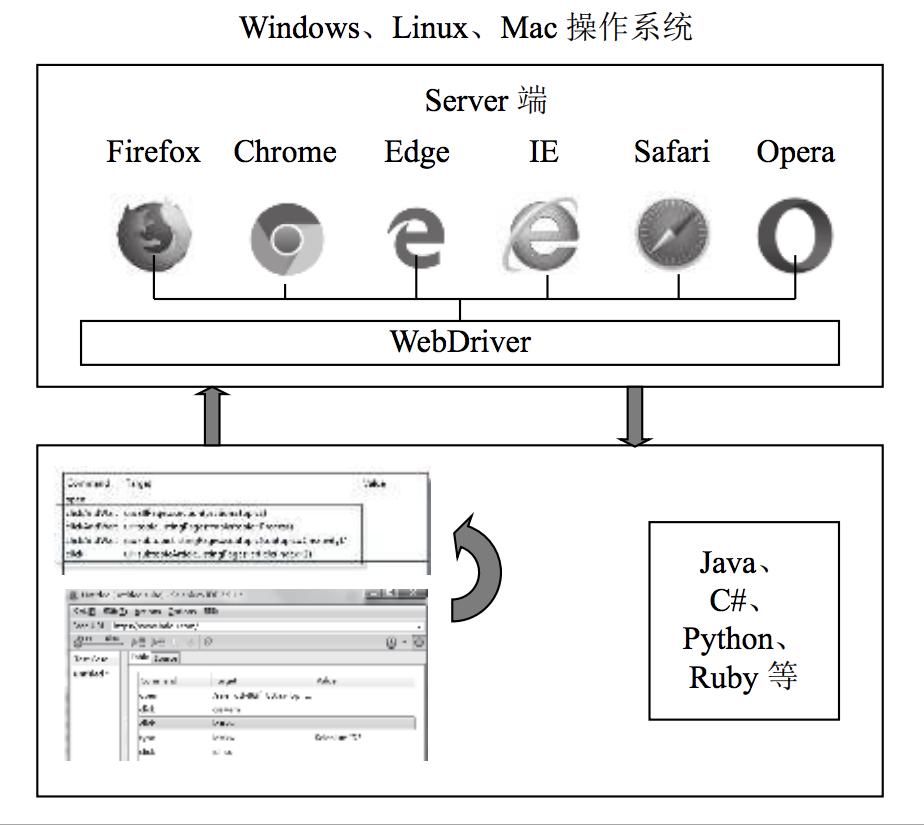
\includegraphics[width=0.68\textwidth]{images/selenium.png}
  \caption{selenium架构图}
  \label{fig:logo}
\end{figure}
\centerline{}


\chapter{恶意爬虫检测技术研究}

\section{爬虫样本与训练数据}
为了检验和评估不同的方案下,爬虫识别算法的检测率和效率,我们使用了三个不同的数据集进行评估。前两个数据集分别为:
\begin{itemize}
\item 清华大学某网站访问数据集 (数据集a)
\item 360天眼恶意攻击流量数据集 (数据集b)
\item 多策略爬虫工具生成数据集 (数据集c)
\end{itemize}

两个数据集的量级均在在10w+左右,其中数据集a记录的是清华大学某重要网站在某时间段内的所有请求。通过基于User-agent的传统方法针对数据集a进行清洗,我们发现基于User-agent的方法识别出请求中的24.3\%为来自各类爬虫的请求,爬虫的组成成分主要是来自于各大搜索引擎的爬虫以及专门针对清华网站的爬虫,如下图所示。因为该数据集几乎不存在对抗样本,因此我们使用ip作为session分类的标准,对全部的10w个请求进行session分类,在去除一些超长和超短的session之后,我们可以得到了以下的session的长度分布。

\centerline{}
\begin{figure}[!h]
  \centering
  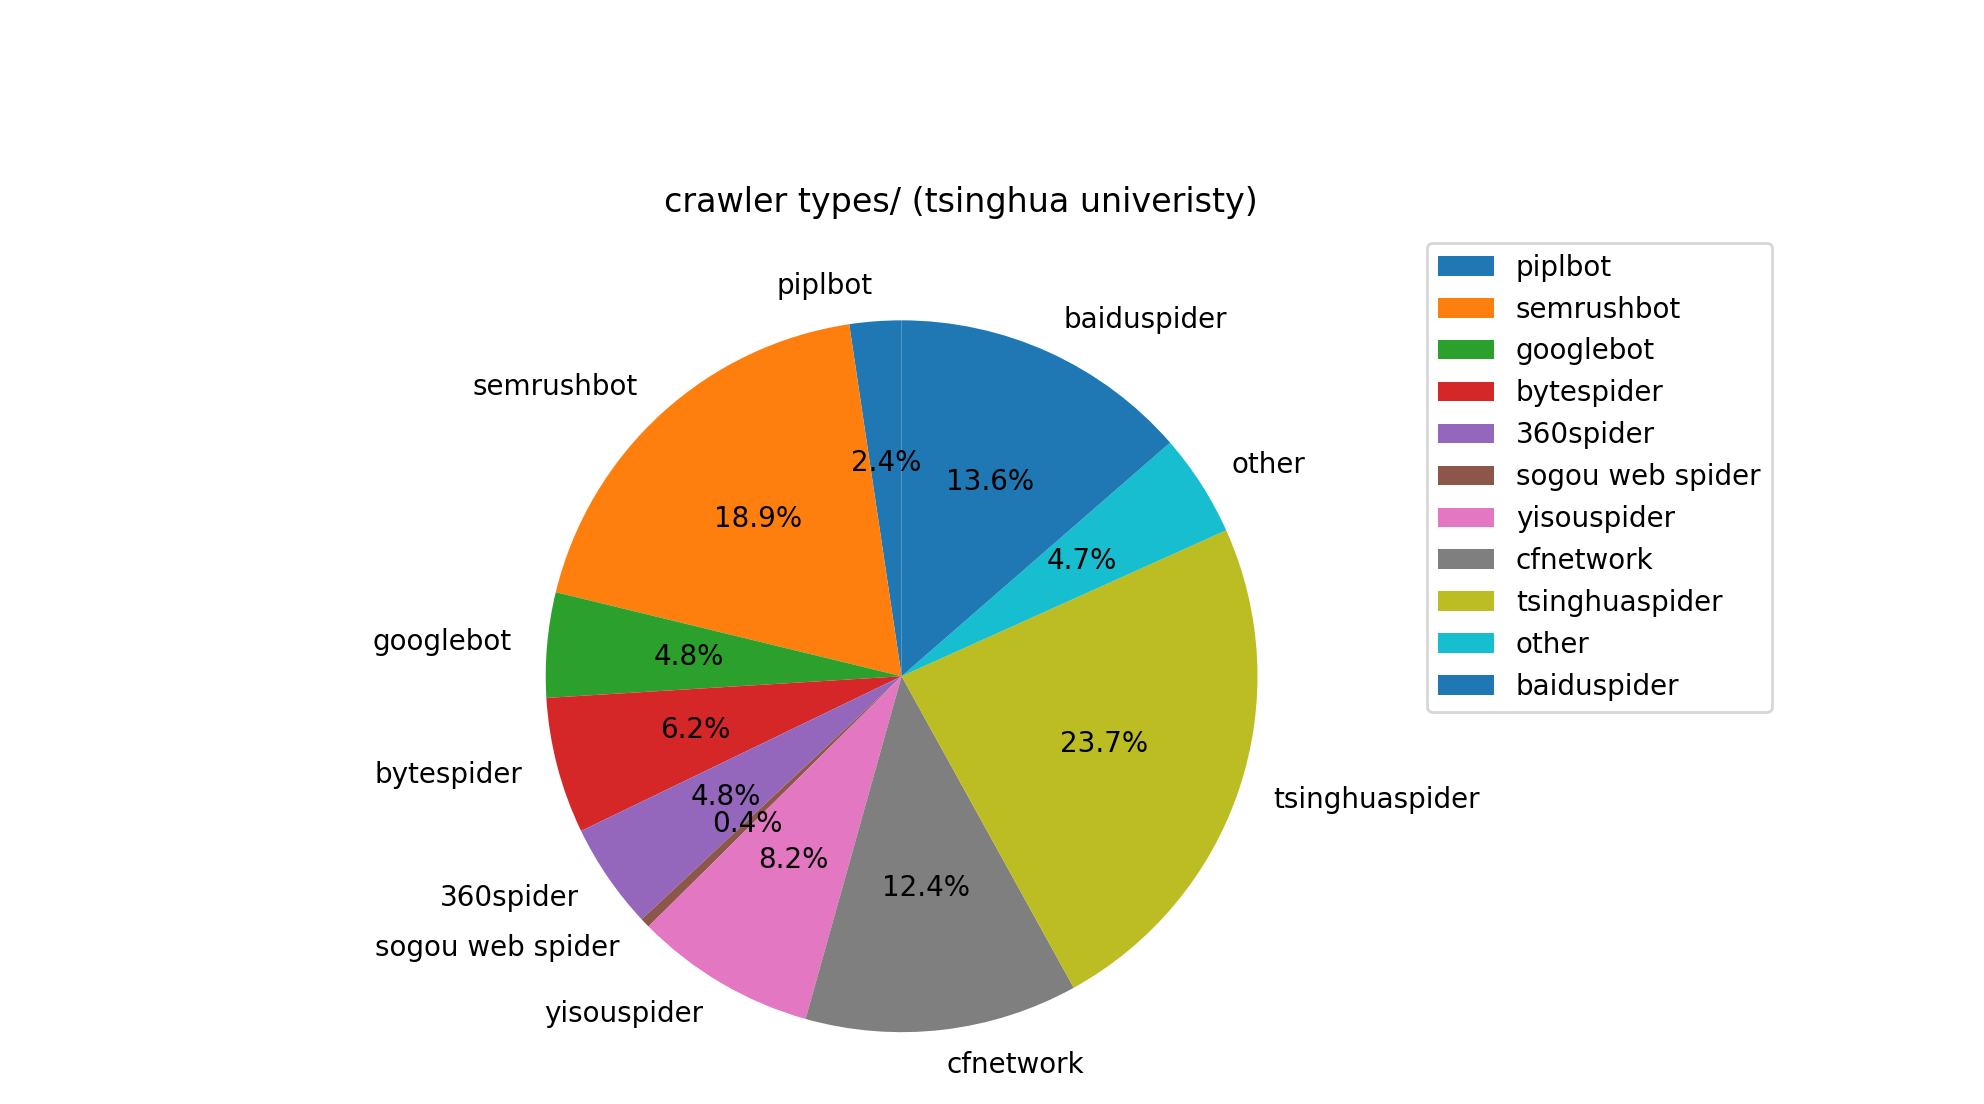
\includegraphics[width=0.68\textwidth]{images/THU_crawler_types.png}
  \caption{清华大学某网站爬虫组成}
  \label{fig:logo}
\end{figure}
\centerline{}

\centerline{}
\begin{figure}[!h]
  \centering
  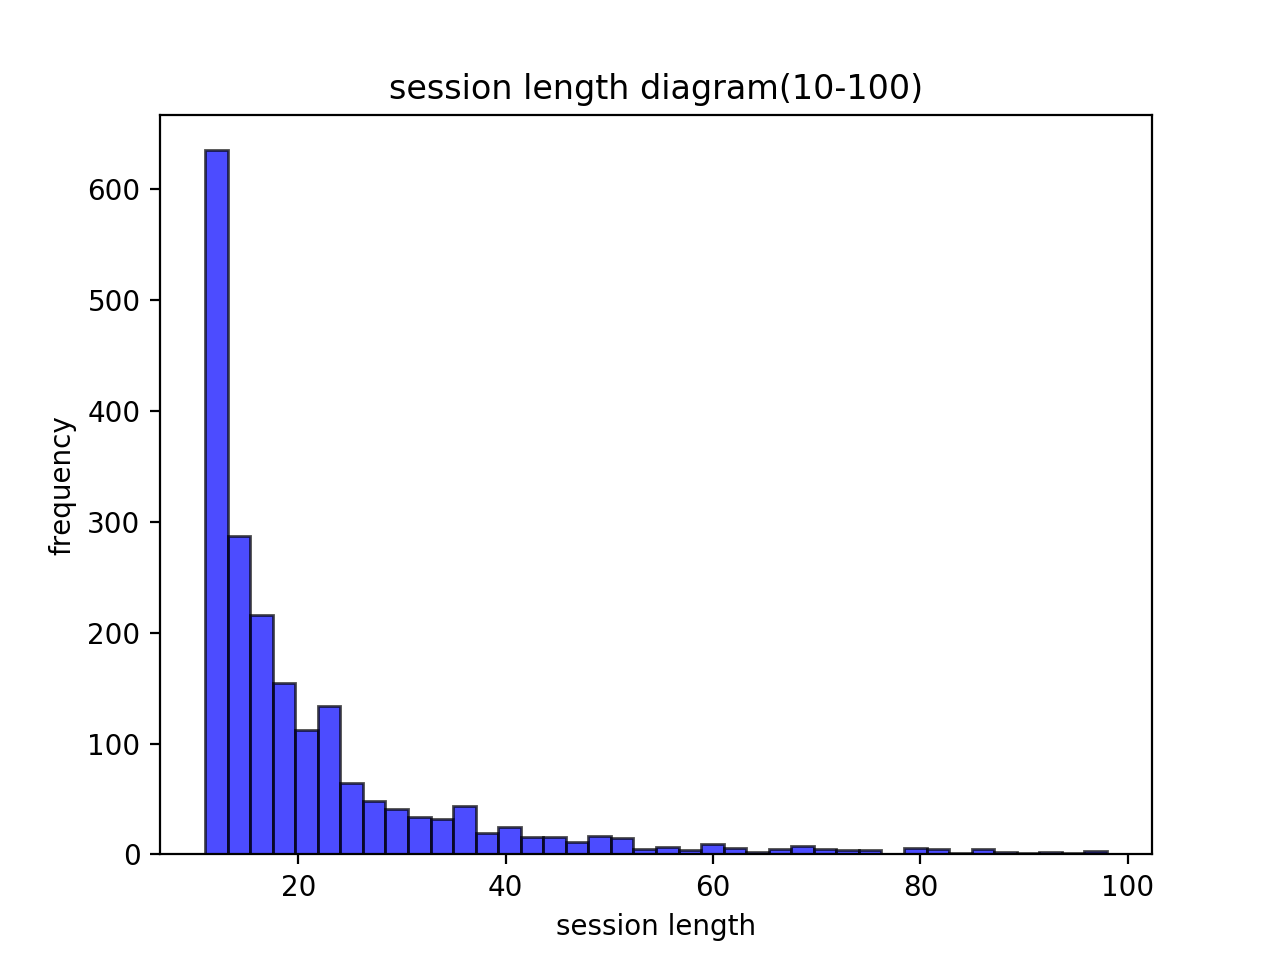
\includegraphics[width=0.68\textwidth]{images/session_len_10_100.png}
  \caption{清华大学某网站访问session长度分布图}
  \label{fig:logo}
\end{figure}
\centerline{}

数据集b来自于360天眼捕获的恶意攻击的流量,这些请求数据绝大部分是互联网上的漏洞扫描爬虫发送的,带有明显的攻击载荷的特征。和传统的爬虫访问流量不同,这些恶意攻击的请求使用了大量的对抗性策略,例如分布式爬取以及http字段变异,通过这些手段,来干扰爬虫识别时的session分类。这对已有论文中,使用session粒度的爬虫检测方法提出了巨大的挑战。该数据集主要应用于验证本文中的session分类方法在遇到遇到对抗性策略的爬虫时,仍能够保持较高的session识别准确率。

但是,静态的访问数据并不能满足我们的需求,因为静态的数据中,缺乏爬虫与服务器之间的交互信息,而在真实情境下,服务器可以通过改变返回的页面中的URL地址,以及返回的javascript代码来影响甚至操纵爬虫的行为。因此,为了模拟真实网络环境中的爬虫请求,我们还设计了一系列的爬虫策略,并基于这些策略,生成了近千种不同类型的网络爬虫,我们称之为多策略爬虫工具。我们考虑到的爬虫特性有:
\begin{itemize}
\item 爬虫的目标数据
\item 爬虫的请求速率
\item 爬虫的遍历算法
\item 爬虫的驱动程序
\item 对抗性的爬虫策略
\end{itemize}

这些不同类型的爬虫将会产生大量普通的爬虫请求以及具有对抗性的爬虫请求,这些爬虫请求在产生的过程中会记录session id用以检测session分类的效果,并且这些爬虫均具有能够执行服务器反馈的javascript的特性,因此可以用于收集不同webdriver下的动态指纹,这些爬虫产生请求将会作为本研究的第三个数据集(数据集c)。


\section{单粒度模式检测规则}
单粒度模式检测指定是在不使用session信息以及动态信息的同时,仅仅利用单个http请求中所有的可用信息,来判定该请求是否源于爬虫的技术。该技术也是应用最广泛、性能消耗最少的爬虫检测方法。因为其对整个系统并没有什么性能损耗,因此在我们的模型和最终的系统中,我们仍然保留单粒度模式检测规则。

在我们的模型中,我们对如下内容进行检测:

\begin{itemize}
\item User-agent字段: User-agent字段主要是访问者的浏览器或者相应的http库标识当前访问者使用的agent的一个重要字段。大部分的普通爬虫,都会在其user-agent字段放置与该爬虫有关的信息,通过该信息,我们可以快速地筛选出这些爬虫。但是,由于user-agent字段是由用户发送的,用户可以随意修改该字段来达到隐蔽真实user-agent的目的,因此,该字段是不可信的。在我们的模型中,通过参考已有的爬虫数据库,我们采用如下的关键字来处理user-agent字段:
    
\centerline{}
\begin{figure}[!h]
  \centering
  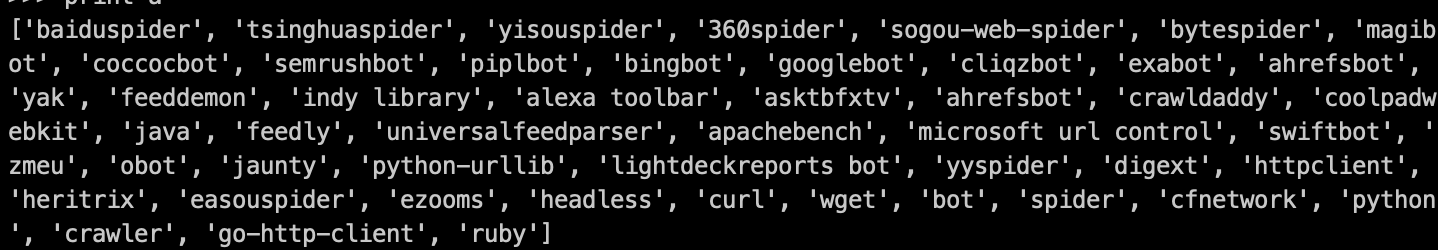
\includegraphics[width=0.68\textwidth]{images/crawler_key_words.png}
  \caption{user-agent关键字}
  \label{fig:logo}
\end{figure}
\centerline{}
    
\item Http 请求方法:http请求方法指的是浏览器等在访问web服务器时,于http请求头中设置的请求方法。常用的请求方法有:HEAD,GET,POST,PUT,OPTIONS等,而正常情况下,浏览器所使用的请求方法只有GET,POST,但是大量的爬虫为了爬取效率常常会使用HEAD方法,部分漏洞扫描器则会使用PUT方法来攻击一些有弱点的服务器(ps: 此处加上引用iis put漏洞 + tomcat put漏洞)。因此,对http请求方法进行判断也能够识别出一部分的爬虫。

\item 特殊的URL地址:部分网站会在网站的web根目录下放置robots.txt,该文件是web服务商与普通爬虫之间的协议,主要的作用便是为爬虫提供一个爬取的规范和限制。如果请求中出现了该url地址,我们即可将该请求标记为爬虫请求。除了robots.txt, 我们在使用后文中出现的taint link技术时,也可能出现会触发一些异常url地址的访问,我们可以将这些标记为爬虫。

\item Http referer:该http请求字段标识着当前请求的访问来源,一般情况下,该referer字段指向的应该是当前网站中存在的某一网页。如果不满足该条件,则标记该请求的来源为爬虫。

\item Http请求中的恶意攻击载荷:在真实的网络环境中,存在着大量漏洞扫描爬虫,这些爬虫发送的请求中往往带有恶意的攻击载荷,通过建立针对攻击载荷的数据库,我们很容易地过滤出这些爬虫。此处,我们参考的攻击载荷数据库来自于360天眼中的规则。详细的规则请参考附录x

\item Http请求头部字段的完备性:通常而言,大部分静态爬虫的主体(如curl以及一些基于python-requests库的简单爬虫)相对于浏览器而言功能负责度角度,这也意味在数据交换中,他们使用的功能字段更少,如下是来源curl的爬虫的访问请求,以及使用chrome的访问请求的完整http数据包的对比
\end{itemize}

\centerline{}
\begin{figure}[!h]
  \centering
  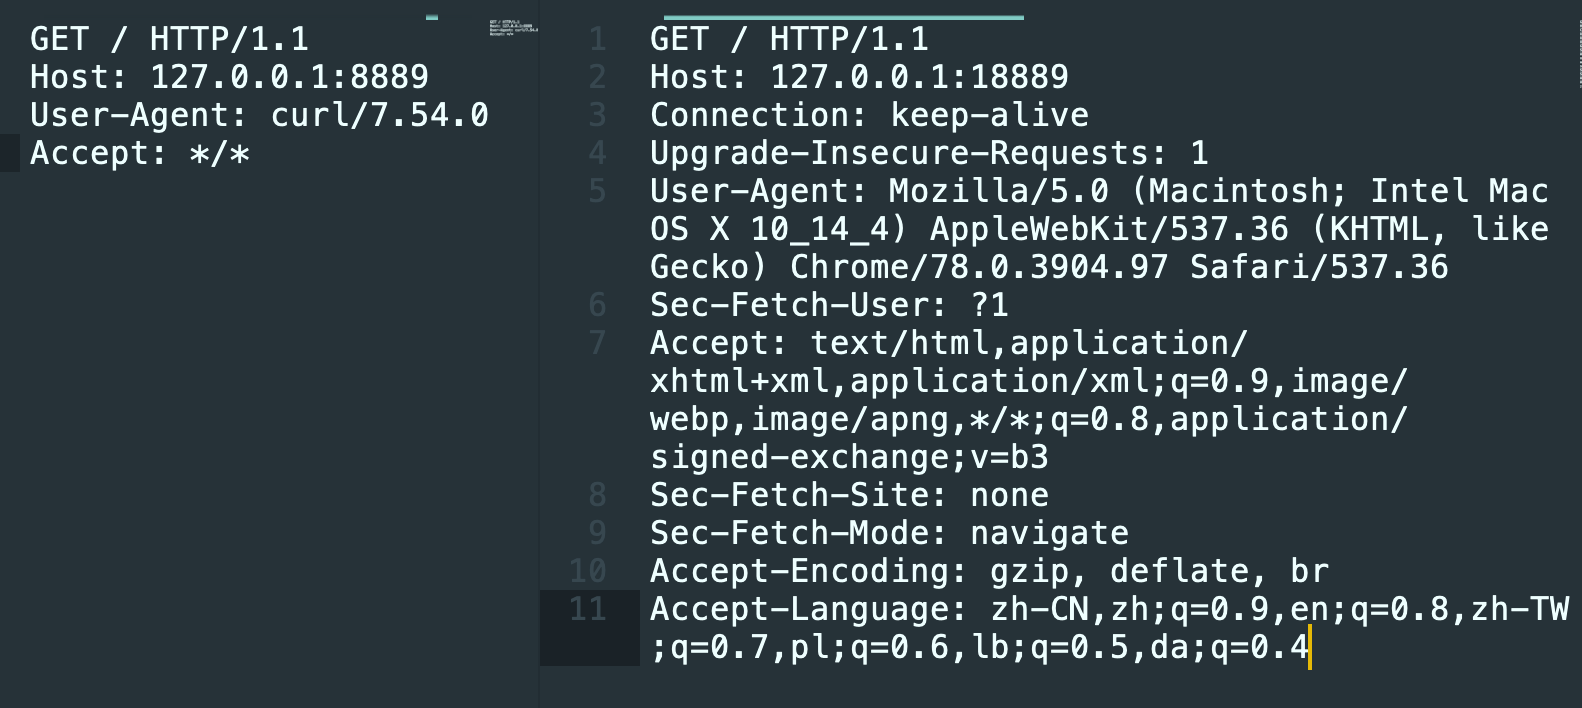
\includegraphics[width=0.68\textwidth]{images/http_request_contrast.png}
  \caption{curl与chrome的访问请求对比}
  \label{fig:logo}
\end{figure}
\centerline{}

由此可以看出两者的http字段的复杂度相差很大。利用这点,我们可以对一些浏览器常用的字段检查,来过滤出一些简单的爬虫。在我们的模型中,我们使用的必要字段是:
Host,Connection,User-Agent,Accept,Accept-Language,Accept-Encoding
没有使用这些字段的请求均会被标记为爬虫。

我们在数据集a和数据集b上使用单粒度模式检测规则的检测效果如下所示:

此处缺图.png


\section{session粒度模式检测}
通过单粒度模式检测,我们可以过滤出互联网上大部分的爬虫。但是,爬虫与反爬虫本质上是一种博弈对抗,一旦爬虫采用一些字段修改和隐藏的方法,去修改我们检查的http特征,那么传统的单粒度模式检测就很发挥应有的作用,因此,我们还需要将我们检测的重点转向那些更难被修改却更加显著特征上,而这些特征主要富集在session粒度层次上。但是,大部分的关于爬虫识别的论文在session分类上都语焉不详,部分论文直接将来自于同ip的请求划分为同一个session,而另一部分论文直接使用cookie来追踪浏览器的session。这种处理显然是无法准确对恶意爬虫进行session分类的,恶意爬虫通常会使用分布式的ip地址,并对cookie部分的字段内容进行伪造,从而欺骗爬虫识别系统。在本节我们将介绍本研究在session分类上采用的策略和方案。

\subsection{静态session分类}
在session分类的处理上,本研究首先采用http字段静态特征作为session分类的依据。主要采用的静态特征有:User-agent字段,URL请求路径,其他header字段,header字段键与其排列顺序。引入header字段排列的主要是基于这样的一个直觉:如果目标爬虫使用了http header字段变异的对抗行为,虽然会改变字段具体的值,但可能忽略对字段键的变异,给该特征赋予较高的权重,能够有效地在此类对抗行为下正确地分类session。在计算两个http请求的相似度时,我们采用如下的计算函数:

$$score = \frac {W_{ua} * M_{ua} + W_{url} * M_{url} + W_{other} * M_{other} + W_{order} * M_{order}} {C_{field} + 2}$$

此处的W为权重相关的系数,M表示相关字段是否匹配,匹配取值为1,反之取值为0,表示相关字段的数目,用以避免字段过多的请求出现评分过高的情况。此外,我们额外设置相应的阈值,一旦相似度超过该阈值,我们即可将两个http请求归类为同一个session。我们在数据集a上测试我们的算法,并使用梯度下降的方法,求得这些参数的较优解。下图是我们使用该静态分类方法效果图(梯度下降图),我们最终采用的参数取值,其分类准确率可以达到88%。

\centerline{}
\begin{figure}[!h]
  \centering
  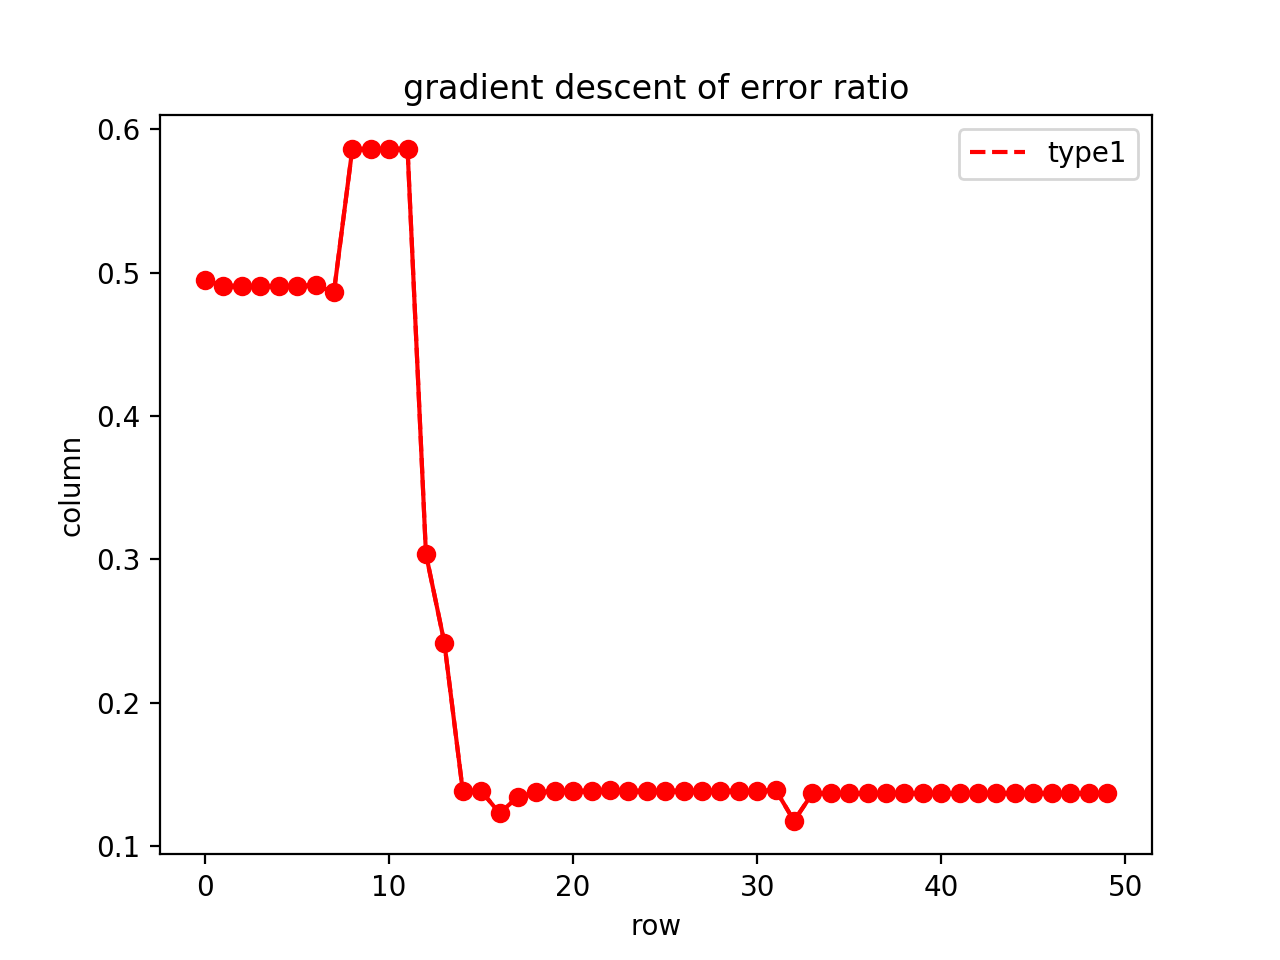
\includegraphics[width=0.68\textwidth]{images/gradient_descent.png}
  \caption{curl与chrome的访问请求对比}
  \label{fig:logo}
\end{figure}
\centerline{}

静态session分类也是在已有的爬虫检测文献中最长使用的方法,但是方法也存在致命的局限性,在面对使用对抗策略的爬虫面前,该session分类方法无法正常地进行分类,下图是静态session方法在三种数据集上的分类效果:

\centerline{}
\begin{table}[h]
  \caption{静态session分类效果比较}
  \label{tab:papercomponents}
  \centering
\begin{tabular}{|p{2cm}<{\centering}||p{5cm}<{\centering}|p{2cm}<{\centering}|p{2cm}<{\centering}|p{2cm}<{\centering}|}
    \hline
    数据集编号 & 数据特性 & 原始session数目 & 分类后session数目 & session分类准确率    \\
    \hline
    a  &  正常用户+普通爬虫 & 100 & 130 & 88\% \\
    \hline
    b  &  恶意漏洞扫描爬虫 & 100 & 291 & 35\% \\
    \hline
     c  & 采用对抗策略的爬虫 & 100 & 472 & 26\% \\
    \hline
    \end{tabular}
\end{table}
\centerline{}


不难看出,在存在对抗样本的数据集b以及数据集c上,静态session分类的准确率都大打折扣。但是如果客户端webdriver开启了javascript执行的功能,那么通过引入动态session分类,能够有效地缓解上述的问题。



\subsection{动态session分类}

\subsubsection{浏览器指纹生成算法}

不同用户的浏览器具有不同的特征信息和丰富的数据,网站可以通过在用户访问时通过不同的 API 和技术手段获取浏览器特征信息构建独特的浏览器指纹。浏览器指纹技术能够在无cookie的情况下提供一种追踪用户的鲁棒性方案。
令指纹生成算法为 F(⋅)。当出现一个新的浏览器信息 x 时,生成一个浏览器指纹 F(x)。该算法遵循离散概率密度函数 P( fn) 。其中,fn 为某个特征信息的指纹生成结果 ;n∈[0,1,…,N],N 为特征信息的个数。对于某单个特征信息的指纹生成结果 fn,使用自信息量 I 表示该浏览器指纹所包含信息的比特数,即:

\begin{equation}
I(F(x)=f_n)=-log_2(P(fn)) \tag{1}
\end{equation}

当指纹由多个不同的特征信息组合而成时,假设不同特征信息对应的指纹生成算法为 Fs(),s∈[0,1,…,S ](S 为指纹生成算法的个数),则根据公式(2)单独计算每个特征信息的指纹生成结果 fn,s 的自信息量 Is(fn,s),并根据公式(3)定义指纹组件的信息熵 Hs(Fs)。

\begin{equation}
I_s(f_{n,s})=-log_2(P(f_{n,s})) \tag{2} 
\end{equation}
\begin{equation}
H_s(F_s)=-\sum_{n=0}^{N}P(f_s,n)log_2(P(f_s,n)) \tag{3}
\end{equation}


信息熵表征浏览器所有自信息量的期望值。对于两个相互独立的特征组件,自信息量可直接线性相加。根据自信息量 I 可以确认指纹归属对象的身份。I 包含的若干比特信息中的每一比特信息都能将该浏览器指纹可能的归属集合减半。特征信息进行组合生成指纹,每一个特征信息具有若干比特的信息熵,熵值越大,则越能准确地区分不同的浏览器实体。因此要选取恰当且包含足够比特信息的特征信息集合,通过该特征信息集合生成的指纹能够唯一确认指纹归属对象的身份。



\subsubsection{Canvas 指纹}
Mowery和Shacham提出了通过HTML 5 的 Canvas API以及WebGL渲染文本得到像素差异,作为一种具有高信息熵的浏览器指纹生成方式[27]。
canvas元素是html5规范中新增的一类元素,能够在屏幕上可编程地绘制图像,并且被大部分主流的浏览器支持。绘制一个基本的canvas图形的方法相当简单:需要浏览器提供给用户一个图形渲染的环境,使用环境中的API来渲染你对canvas图像的操作和改变。在目前使用的html5规范中,广泛使用的2d环境能提供诸如fillRect, lineTo以及arc这样的一些基本绘图功能。也有一些复杂的功能可以支持贝塞尔曲线,颜色梯度的这样一些功能。

\begin{itemize}
\item Canvas Text渲染:给定字体,字体颜色以及位置参数,2d context能够在canvas绘制出任意的文本。
\item Canvas 像素抽取: 2D context提供了一个getImageData方法,通过该方法能够获取一个给定区域范围内的图片对象,该对象是以图片中的每一个元素的RGBA值组成的。其次,canvas对象本身提供toDataURL方法,当提供一个图片作为该方法的输入后,该方法能够将完整的图片内容以base64编码的形式返回。以上两个方法均严格遵循浏览器同源策略。
\item WebFront:webFront是定义在CSS3中的规范,允许用户按需加载远程字体,而不是只能依赖于已经安装在本地的字体。在使用这个特性时,需要加入@front-face这样一条规则,并使用src属性指定远程字体资源的url地址。为了使用WebFront,需要开启WebFront Loader函数库。通过使用该函数库,WebFront仅仅通过JavaScript就能够加载。
 \item WebGL:WebGL提供了一个javascript的API用于在canvas上绘制图像,目前的主流浏览器都支持WebGL的硬件加速选项,可以使用图形硬件来渲染每一帧,目前WebGL也通过各自的canvas环境暴露出相应的函数接口,类似于OpenGL API,可以使用GLSL(OpenGL Shading Language)编程,在编译后,可以直接运行在硬件显卡上。
 \end{itemize}


\subsubsection{浏览器特定指纹}
ECKERSLEY根据浏览器的环境,通过收集一些网站能够获取的浏览器常用或者不常用的特性,用以生成浏览器的指纹[26]。这些特性中有一部分可以通过简单静态的HTTP请求中推断出来,也可以经由AJAX接口收集。特性收集过程中,有一部分特性是简单明了的,但有一部分特性是来源于一些浏览器细节。有些浏览器禁用了javascript,那么他会使用video,plugins,fonts和supercookie的默认值。因此可以通过这一细节来推断出浏览器是否禁用了javascript。我们在研究中使用了如下的常见浏览器特性来产生浏览器指纹:

\begin{itemize}
\item user-agent
\item 浏览器语言设置
\item 浏览器storage设置 (SessionStorage,LocalStorage,IndexDb)
\item cookie支持
\item 屏幕分辨率
\item timezone
\item 浏览器插件信息
\item 系统字体
\item doNotTrack标识
\item ie activex支持
\item canvas指纹
 \end{itemize}
 
 以下是我们在不同操作系统,不同版本的不同浏览器上根据以上特征使用hash算法生成的128 bit指纹。
 
\centerline{}
\begin{table}[h]
  \caption{不同浏览器指纹比较}
  \label{tab:papercomponents}
  \centering
\begin{tabular}{|p{3cm}<{\centering}||p{3cm}<{\centering}|p{3cm}<{\centering}|p{6cm}<{\centering}|}
    \hline
    webdriver名称 & 版本 & 操作系统 & 浏览器指纹    \\
    \hline
   
chromium & 70.0.3509.0 & ubuntu 16.04 x64 & 1a82cc57a97d7a931a82cc5720de9977 \\
\hline
chromium & 70.0.3514.0 & ubuntu 16.04 x64 & bae33d459368bee9bae33d45b8a2efa1\\
\hline
chromium & 70.0.3519.0 & ubuntu 16.04 x64 & 06a3007b36556ee506a3007bad572654\\
\hline
firefox(headless) & 57 & ubuntu 16.04 x64 & 576d92810cef4933576d9281c52a137b\\
\hline
firefox(headless) & 63 & ubuntu 16.04 x64 & 332ac9f169afb00b332ac9f18b81828d\\
\hline
firefox(headless) & 68 & ubuntu 16.04 x64 & 4cb3ae543ab898494cb3ae54fc189ce4\\
\hline
phantomjs & 1.9.7 & ubuntu 16.04 x64 & 2d15aa2ba520737e2d15aa2b4a84aa17\\
\hline
phantomjs & 1.9.8 & ubuntu 16.04 x64 & 4c83cbcb790af6734c83cbcb8e935880\\
\hline
phantomjs & 2.1.1 & ubuntu 16.04 x64 & ba8506ab17e80837ba8506ab62082282\\
\hline
chrome & 78.0.3904.97 & macos 10.14.4 & 49c81cf7b7d05f9e49c81cf71fce9c5e\\
\hline
safari & 12.1 & macos 10.14.4 & 410160ac93cefc91410160ac72900fc9\\
\hline
firefox & 70.0.1 & macos 10.14.4 & 259295adde33bc05259295ad81fa3bed\\
\hline
chrome & 78.0.3904.84 & ios 12.2 & cef500876945eee2cef50087fadd5d18\\
\hline
    \end{tabular}
\end{table}
\centerline{}

根据Mowery的论文[12],动态指纹的独特性和熵能够得到保证。因此,在并发流量不太高的情况下,将其作为session分类的重要依据,能够得到相当高的准确率。我们将动态指纹加入到我们的相似度计算函数,函数更新后为:

$$score = \frac {W_{ua} * M_{ua} + W_{url} * M_{url} + W_{other} * M_{other} + W_{order} * M_{order} + W_{dynamic} * M_{dynamic}} {C_{field} + 3}$$

因为我们使用的动态指纹分类技术需要javascript的支持,原先的数据集a和b并没有记录下相关的信息,因此我们只能使用数据集c来作为评估基于静态/动态指纹的session分类方法的准确性。在动态指纹生成的整个过程,我们首先在请求中捕获没有动态指纹生成、动态指纹过期、动态指纹伪造的请求,针对该请求发送相应的指纹生成javascript脚本脚本执行完后,会产生浏览器的特定指纹,并将该指纹返回到服务器(最好使用加密算法),服务器根据该指纹,分配并绑定session。大致流程如下图所示:


\centerline{}
\begin{figure}[!h]
  \centering
  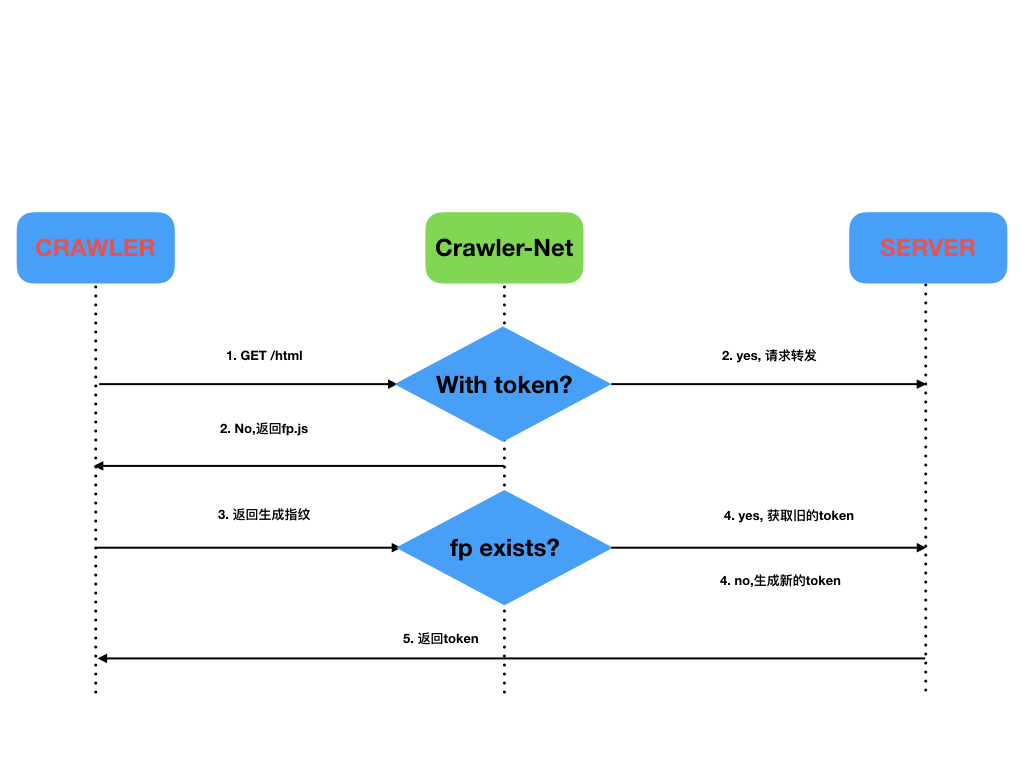
\includegraphics[width=0.68\textwidth]{images/fingerprint_generation.jpg}
  \caption{浏览器指纹生成流程}
  \label{fig:logo}
\end{figure}
\centerline{}

最终结果显示,我们的准确率是96.71\%,而静态指纹的session分类算法在数据集c上的准确率仅仅为23.73\%。


\subsection{session检测规则}

结合已有论文中的方法以及我们的具体使用场景,在session检测规则上,我们主要考虑如下特征:

\begin{itemize}
\item 4xx/5xx 返回状态码的比例:http返回的状态码指示了当前http请求处理结果的状态。最常见的正常返回时200,对应的返回状态是”OK“,在提交登录凭证的时候,也有可能产生一些从定向的返回状态码,如301和302。而出现4xx以及5xx的状态码时,往往以为这服务器在处理相关请求时出现了错误,或者用户发送的http请求并不是一个满足http协议的合法的请求。在普通的用户用浏览器访问的情况下,很少会出现这样的状态。而爬虫因为其扩张性以及一定的侵略性,则经常会触发相应的错误,尤其是因为访问服务器上不存在的资源而触发”404 not found“的错误。
\item 某时间段内(如1min)内的最大请求次数:高频率地请求网站的相关资源,从而导致web服务器的带宽资源以及计算资源被大量消耗,是恶意爬虫对网站的主要危害之一,而普通用户的访问往往是达不到很高的请求速率的。因此某段时间内的最大请求频次可以作为一个关键指标,来衡量一个session是否来自于爬虫。
\item 请求时间间隔标准差:爬虫的请求频率和次数往往由程序事先定义好,因此从session角度来看,爬虫的请求时间间隔通常会有很强的规律性,而这些时间间隔的标准差,正是能够反应该规律性显著程度的重要指标。
\item 请求URL资源不同类型比例:爬虫访问与人类访问相比,更加注重数据的收集和效率,而人类更注重数据的可读性。基于这种假设,我们不难得出结论,爬虫对于web page资源更加偏爱,但是会忽略一部分对于爬虫而言没有意义的样式表文件,字体文件,javascript文件的加载。因此,根据session中的url资源比例,能够判定出一部分的爬虫。
\end{itemize}

如下,是从数据集a中抽取了具有代表性的爬虫session以及人类session的特征比较:




% 说明
% !TeX root = ../Template.tex
% 本LaTeX模板的一般使用说明
\chapter{说明}

Again,这是北航论文\LaTeX{}模板(\CTeX{}-Based)\BUAAThesis{}。

本\LaTeX{}模板为北航研究生学位论文模板,适用于理工类博士、学术硕士和专业硕士。本\LaTeX{}模板参考自2015年8月版北航《研究生手册》,具体要求请参见各自的《手册》,最终成文格式需参考学院要求及打印方意见。本模板中大量内容和说明直接摘抄自《手册》(2015年8月版),基本覆盖了论文内容和格式方面的要求。

本模板已上传\href{https://github.com/CheckBoxStudio/BUAAThesis}{GitHub},该仓库中同时也包含了相应的Word模板。

%-----------------------------
\section{宏包使用}

请将以下文件与此LaTeX文件放在同一目录中:

\begin{tabular}{ll}
 \verb|buaa.cls |             & $\triangleright$ LaTeX宏模板文件 \\
 \verb|buaa_mac.cls |         & $\triangleright$ LaTeX宏模板文件(For Mac with XeLaTeX) \\
 \verb|GBT7714-2005.bst|      & $\triangleright$ 国标参考文献BibTeX样式文件2005 \\
 \verb|GBT7714-2015.bst|      & $\triangleright$ 国标参考文献BibTeX样式文件2015 \\
 \verb|logo-buaa.eps|         & $\triangleright$ 论文封皮北航字样 \\
 \verb|head-doctor.eps|       & $\triangleright$ 论文封皮北博士学位论文标题\\
 \verb|head-master.eps|       & $\triangleright$ 论文封皮北学硕学位论文标题 \\
 \verb|head-professional.eps| & $\triangleright$ 论文封皮北专硕学位论文标题\\
 \verb|tex/*.tex|             & $\triangleright$ 本模板样例中的独立章节\\
\end{tabular}\\

通过 \verb|\documentclass[<thesis>,<permission>,<printtype>,<ctexbookoptions>]{buaa}|载入宏包:
\begin{itemize}[leftmargin=3cm]
  \item[{\tt thesis} $\triangleright$]  论文类型(thesis),可选值:\\
    a) 学术硕士论文(\verb|master|)[缺省值]\\
    b) 专业硕士论文(\verb|professional|)\\
    c) 博士论文(\verb|doctor|)
  \item[{\tt permission} $\triangleright$] 密级(permission),可选值: \\
    a) 公开(\verb|public|)[缺省值]\\
    b) 内部(\verb|privacy|)\\
    c) 秘密(\verb|secret|=\verb|secret3|)\\
    --- c.1) 秘密3年(\verb|secret3|)\\
    --- c.2) 秘密5年(\verb|secret5|)\\
    --- c.3) 秘密10年(\verb|secret10|)\\
    --- c.4) 秘密永久(\verb|secret*|)\\
    d) 机密(\verb|classified|=\verb|classified5|)\\
    --- d.1) 机密3年(\verb|classified3|)\\
    --- d.2) 机密5年(\verb|classified5|)\\
    --- d.3) 机密10年(\verb|classified10|)\\
    --- d.4) 机密永久(\verb|classified*|)\\
    e) 绝密(\verb|topsecret|=\verb|topsecret10|)\\
    --- e.1) 绝密3年(\verb|topsecret3|)\\
    --- e.2) 绝密5年(\verb|topsecret5|)\\
    --- e.3) 绝密10年(\verb|topsecret10|)\\
    --- e.4) 绝密永久(\verb|topsecret*|)
  \item[{\tt printtype} $\triangleright$] 打印属性(printtype),可选值: \\
    a) 单面打印(\verb|oneside|)[缺省值]\\
    b) 双面打印(\verb|twoside|)
  \item[{\tt ctexbookoptions} $\triangleright$] {\tt ctexbook}文档类支持的其他选项: \\
    使用{\tt ctexbookoptions}选项传递{\tt ctexbook}文档类支持的其他选项。
    例如,使用{\tt fontset=founder}选项启用方正字体以避免生僻字乱码的问题\footnote{需要系统安装方正字体。}。
\end{itemize}

模板已内嵌LaTeX工具包:
 {\tt ifthen},{\tt etoolbox},{\tt titletoc},{\tt remreset},{\tt remreset},
 {\tt geometry},{\tt fancyhdr},{\tt setspace},{\tt caption},{\tt float},
 {\tt graphicx},{\tt subfigure},{\tt epstopdf},
 {\tt book\-tabs},{\tt longtable},{\tt multirow},{\tt array}, {\tt enumitem},
 {\tt algorithm2e},{\tt amsmath},{\tt amsthm},{\tt listings},
 {\tt pifont},{\tt color},{\tt soul}, {\tt newtxtext}, {\tt newtxmath}。

模板已内嵌宏:\verb|\highlight{text}|(黄色高亮)。

请统一使用UTF-8编码。



%-----------------------------
\section{选项设置}

\begin{itemize}[leftmargin=3cm]
  \item[{\tt  $\backslash$refcolor} $\triangleright$]  开启/关闭引用编号颜色,包括参考文献,公式,图,表,算法等\\
  \texttt{on}:开启 [默认]\\
  \texttt{off}:关闭
  \item[{\tt $\backslash$beginright} $\triangleright$]  摘要和正文从右侧开始\\
  \texttt{on}:开启 [默认]\\
  \texttt{off}:关闭
  \item[{\tt $\backslash$emptypageword} $\triangleright$]  空白页留字
  \item[{\tt $\backslash$Listfigtab} $\triangleright$]  是否使用图标清单目录\\
  \texttt{on}:开启 [默认]\\
  \texttt{off}:关闭
\end{itemize}


%-----------------------------
\section{章节撰写}
本模板支持以下标题级别标题级别:

\begin{tabular}{ll}
  \verb|\chapter{章}|              & $\triangleright$ 第一章 \\
  \verb|\chapter*{无章号章}|       & $\triangleright$ 无章号章 \\
  \verb|\chaptera{无章号有目录章}| & $\triangleright$ 无章号有目录章 \\
  \verb|\summary|                  & $\triangleright$ 总结\\
  \verb|\appendix|                 & $\triangleright$ 附录\\
  \verb|\achievement|              & $\triangleright$ 攻读学位期间取得的成果\\
  \verb|\acknowledgments|          & $\triangleright$ 致谢\\
  \verb|\biography|                & $\triangleright$ 作者简介\\
  \verb|\section{节}|              & $\triangleright$ 1.1 节\\
  \verb|\subsection{条}|           & $\triangleright$ 1.1.1 条\\
  \verb|\subsubsection{A}|         & $\triangleright$ 1.1.1.1 A\\
  \verb|\paragraph{a}|             & $\triangleright$ 1.1.1.1.1 a\\
  \verb|\subparagraph{a)}|         & $\triangleright$ 1.1.1.1.1.1 a)\\
\end{tabular}

%-----------------------------
\section{注意事项}
\begin{itemize}
  \item[$\triangleright$] \textit{中文斜体}将转换为楷体;
  \item[$\triangleright$] \verb|buaa.cls|采用包{\tt newtxtext}和{\tt newtxmath},\textbf{中文粗体}在Windows下转换为黑体(有可能是因为newtx包没安装好,By WeiQM),Linux下正常(By QiaoJF);
  \item[$\triangleright$] \verb|buaa_mac.cls|采用包{\tt times},\textbf{中文粗体}转换为黑体(By CaiBW);
  \item[$\triangleright$] \verb|\label{<text>}|中不能使用中文;
  \item[$\triangleright$] 浮动体与正文之间的距离是弹性的;
  \item[$\triangleright$] 命令符与汉字之间请注意加空格以避免undefined错误(pdfLaTeX下好像一般不存在这个问题,主要在XeLaTeX编译环境下发生);
\end{itemize}

%-----------------------------
\section{ToDo}
\begin{itemize}
  \item[$\triangleright$] 数学环境的行间隔;
  \item[$\triangleright$] 参考文献的行间隔;
\end{itemize}

%-----------------------------
\section{意见及问题反馈}

\indent E-mail:weiqm@buaa.edu.cn

\indent GitHub:\href{https://github.com/CheckBoxStudio/BUAAThesis/issues}{https://github.com/CheckBoxStudio/BUAAThesis/issues}


% 示例
% !TeX root = ../Template.tex
% 本LaTeX模板的使用示例
\chapter{示例}

%==============================
\section{参考文献引用}

%--------------------------------
\subsection{数字标注}
\noindent
\begin{tabular}{l@{\quad$\Rightarrow$\quad}l}
  \verb|\cite{knuth86a}| & \cite{knuth86a}\\
  \verb|\citet{knuth86a}| & \citet{knuth86a}\\
  \verb|\citet[chap.~2]{knuth86a}| & \citet[chap.~2]{knuth86a}\\[0.5ex]
  \verb|\citep{knuth86a}| & \citep{knuth86a}\\
  \verb|\citep[chap.~2]{knuth86a}| & \citep[chap.~2]{knuth86a}\\
  \verb|\citep[see][]{knuth86a}| & \citep[see][]{knuth86a}\\
  \verb|\citep[see][chap.~2]{knuth86a}| & \citep[see][chap.~2]{knuth86a}\\[0.5ex]
  \verb|\citet*{knuth86a}| & \citet*{knuth86a}\\
  \verb|\citep*{knuth86a}| & \citep*{knuth86a}\\
\end{tabular}
\par\noindent
\begin{tabular}{l@{\quad$\Rightarrow$\quad}l}
  \verb|\citet{knuth86a,tlc2}| & \citet{knuth86a,tlc2}\\
  \verb|\citep{knuth86a,tlc2}| & \citep{knuth86a,tlc2}\\
  \verb|\cite{knuth86a,knuth84}| & \cite{knuth86a,knuth84}\\
  \verb|\upcite{knuth86a,knuth84}| & \upcite{knuth86a,knuth84}\\
  \verb|\citet{knuth86a,knuth84}| & \citet{knuth86a,knuth84}\\
  \verb|\citep{knuth86a,knuth84}| & \citep{knuth86a,knuth84}\\
  \verb|\cite{knuth86a,knuth84,tlc2}| & \cite{knuth86a,knuth84,tlc2}\\
\end{tabular}

%--------------------------------
\subsection{数字标注-上标形式}
\noindent
\begin{tabular}{l@{\quad$\Rightarrow$\quad}l}
  \verb|\upcite{knuth86a}| & \upcite{knuth86a}\\
  \verb|\upcite{knuth86a,knuth84,tlc2}| & \upcite{knuth86a,knuth84,tlc2}\\
\end{tabular}
\par\noindent
实现源码:\verb|\newcommand{\upcite}[1]{\textsuperscript{\cite{#1}}}|。


%--------------------------------
\subsection{著者-出版年制标}
\citestyle{authoryear}
\noindent
\begin{tabular}{l@{\quad$\Rightarrow$\quad}l}
  \verb|\cite{knuth86a}| & \cite{knuth86a}\\
  \verb|\citet{knuth86a}| & \citet{knuth86a}\\
  \verb|\citet[chap.~2]{knuth86a}| & \citet[chap.~2]{knuth86a}\\[0.5ex]
  \verb|\citep{knuth86a}| & \citep{knuth86a}\\
  \verb|\citep[chap.~2]{knuth86a}| & \citep[chap.~2]{knuth86a}\\
  \verb|\citep[see][]{knuth86a}| & \citep[see][]{knuth86a}\\
  \verb|\citep[see][chap.~2]{knuth86a}| & \citep[see][chap.~2]{knuth86a}\\[0.5ex]
  \verb|\citet*{knuth86a}| & \citet*{knuth86a}\\
  \verb|\citep*{knuth86a}| & \citep*{knuth86a}\\
\end{tabular}
\par\noindent
\begin{tabular}{l@{\quad$\Rightarrow$\quad}l}
  \verb|\citet{knuth86a,tlc2}| & \citet{knuth86a,tlc2}\\
  \verb|\citep{knuth86a,tlc2}| & \citep{knuth86a,tlc2}\\
  \verb|\cite{knuth86a,knuth84}| & \cite{knuth86a,knuth84}\\
  \verb|\citet{knuth86a,knuth84}| & \citet{knuth86a,knuth84}\\
  \verb|\citep{knuth86a,knuth84}| & \citep{knuth86a,knuth84}\\
\end{tabular}
\citestyle{numbers}

%--------------------------------
\subsection{其他形式的标注}
\noindent
\begin{tabular}{l@{\quad$\Rightarrow$\quad}l}
  \verb|\citealt{tlc2}| & \citealt{tlc2}\\
  \verb|\citealt*{tlc2}| & \citealt*{tlc2}\\
  \verb|\citealp{tlc2}| & \citealp{tlc2}\\
  \verb|\citealp*{tlc2}| & \citealp*{tlc2}\\
  \verb|\citealp{tlc2,knuth86a}| & \citealp{tlc2,knuth86a}\\
  \verb|\citealp[pg.~32]{tlc2}| & \citealp[pg.~32]{tlc2}\\
  \verb|\citenum{tlc2}| & \citenum{tlc2}\\
  \verb|\citetext{priv.\ comm.}| & \citetext{priv.\ comm.}\\
\end{tabular}

\noindent
\begin{tabular}{l@{\quad$\Rightarrow$\quad}l}
  \verb|\citeauthor{tlc2}| & \citeauthor{tlc2}\\
  \verb|\citeauthor*{tlc2}| & \citeauthor*{tlc2}\\
  \verb|\citeyear{tlc2}| & \citeyear{tlc2}\\
  \verb|\citeyearpar{tlc2}| & \citeyearpar{tlc2}\\
\end{tabular}

\section{浮动体}

\section{算法环境}

模板中使用 \texttt{algorithm2e} 宏包实现算法环境。关于该宏包的具体用法请阅读宏包的官方文档。\\
\centerline{-----------$\downarrow$-----------Space Check-----------$\downarrow$-----------}

\begin{algorithm}[!h]
  %\SetAlgoLined
  %\SetAlgoVlined
  \caption{A How to (plain).}
  \KwData{this text}
  \KwResult{how to write algorithm with \LaTeX2e{} }
  
  initialization\;
  \While{not at end of this document}{
    read current\;
    \eIf{understand}{
      go to next section\;
      current section becomes this one\;
    }{
      go back to the beginning of current section\;
    }
  }
\end{algorithm}

\centerline{-----------$\uparrow$-----------Space Check-----------$\uparrow$-----------}

\RestyleAlgo{ruled}
\begin{algorithm}[!h]
  \caption{A How to (ruled).}
  \KwData{this text}
  \KwResult{how to write algorithm with \LaTeX2e{} }
  
  initialization\;
  \While{not at end of this document}{
    read current\;
    \eIf{understand}{
      go to next section\;
      current section becomes this one\;
    }{
      go back to the beginning of current section\;
    }
  }
\end{algorithm}

\RestyleAlgo{boxed}
\begin{algorithm}[!h]
  \caption{A How to (boxed).}
  \KwData{this text}
  \KwResult{how to write algorithm with \LaTeX2e{} }
  
  initialization\;
  \While{not at end of this document}{
    read current\;
    \eIf{understand}{
      go to next section\;
      current section becomes this one\;
    }{
      go back to the beginning of current section\;
    }
  }
\end{algorithm}

\RestyleAlgo{boxruled}
\begin{algorithm}[!h]
  \caption{A How to (boxruled).}
  \KwData{this text}
  \KwResult{how to write algorithm with \LaTeX2e{} }
  
  initialization\;
  \While{not at end of this document}{
    read current\;
    \eIf{understand}{
      go to next section\;
      current section becomes this one\;
    }{
      go back to the beginning of current section\;
    }
  }
\end{algorithm}

\subsection{三线表}
推荐使用三线表的方式,如表~\ref{tab:exampletable}。\\
\centerline{-----------$\downarrow$-----------Space Check-----------$\downarrow$-----------}

\begin{table}[!h]
  \centering
  \caption{表的标题}
  \label{tab:exampletable}
  \begin{tabular}{p{4cm}p{4cm}}
    \toprule
    \multicolumn{1}{c}{\textbf{操作系统}} & \multicolumn{1}{c}{\textbf{TeX 发行版}} \\
    \midrule
    所有 & TeX Live \\
    macOS & MacTeX \\
    Windows & MikTeX \\
    \bottomrule
  \end{tabular}
\end{table}

\begin{table}[!h]
  \centering
  \caption{让我们看看一个长标题长什么样。还不够长?那我再多写一点。还是不够长?那我再多写一点点。OK,就是长这样的!}
  \label{tab:exampletable}
  \begin{tabular}{p{4cm}p{4cm}}
    \toprule
    \multicolumn{1}{c}{\textbf{操作系统}} & \multicolumn{1}{c}{\textbf{TeX 发行版}} \\
    \midrule
    所有 & TeX Live \\
    macOS & MacTeX \\
    Windows & MikTeX \\
    \bottomrule
  \end{tabular}
\end{table}

\centerline{-----------$\uparrow$-----------Space Check-----------$\uparrow$-----------}

我们在这儿插入一行字;

我们在这儿再插入一行字;

我们在这儿插入一行字;

我们在这儿再插入一行字;

我们在这儿插入一行字;

我们在这儿再插入一行字;

我们在这儿插入一行字;

我们在这儿再插入一行字;

\section{长表格}

超过一页的表格要使用专门的 \texttt{longtable} 环境(表~\ref{tab:longtable})。\\
\centerline{-----------$\downarrow$-----------Space Check-----------$\downarrow$-----------}


\begin{longtable}[h]{ccc}
  % 首页表头
  \caption[长表格演示]{长表格演示}
  \label{tab:longtable}\\
  \toprule
  名称  & 说明 & 备注\\
  \midrule
  \endfirsthead
  % 续页表头
  \caption[]{长表格演示(续)} \\
  \toprule
  名称  & 说明 & 备注 \\
  \midrule
  \endhead
  % 首页表尾
  \hline
  \multicolumn{3}{r}{\small 续下页}
  \endfoot
  % 续页表尾
  \bottomrule
  \endlastfoot
  
  AAAAAAAAAAAA   &   BBBBBBBBBBB   &   CCCCCCCCCCCCCC   \\
  AAAAAAAAAAAA   &   BBBBBBBBBBB   &   CCCCCCCCCCCCCC   \\
  AAAAAAAAAAAA   &   BBBBBBBBBBB   &   CCCCCCCCCCCCCC   \\
  AAAAAAAAAAAA   &   BBBBBBBBBBB   &   CCCCCCCCCCCCCC   \\
  AAAAAAAAAAAA   &   BBBBBBBBBBB   &   CCCCCCCCCCCCCC   \\
  AAAAAAAAAAAA   &   BBBBBBBBBBB   &   CCCCCCCCCCCCCC   \\
  AAAAAAAAAAAA   &   BBBBBBBBBBB   &   CCCCCCCCCCCCCC   \\
  AAAAAAAAAAAA   &   BBBBBBBBBBB   &   CCCCCCCCCCCCCC   \\
  AAAAAAAAAAAA   &   BBBBBBBBBBB   &   CCCCCCCCCCCCCC   \\
  AAAAAAAAAAAA   &   BBBBBBBBBBB   &   CCCCCCCCCCCCCC   \\
  AAAAAAAAAAAA   &   BBBBBBBBBBB   &   CCCCCCCCCCCCCC   \\
  AAAAAAAAAAAA   &   BBBBBBBBBBB   &   CCCCCCCCCCCCCC   \\
  AAAAAAAAAAAA   &   BBBBBBBBBBB   &   CCCCCCCCCCCCCC   \\
  AAAAAAAAAAAA   &   BBBBBBBBBBB   &   CCCCCCCCCCCCCC   \\
  AAAAAAAAAAAA   &   BBBBBBBBBBB   &   CCCCCCCCCCCCCC   \\
  AAAAAAAAAAAA   &   BBBBBBBBBBB   &   CCCCCCCCCCCCCC   \\
  AAAAAAAAAAAA   &   BBBBBBBBBBB   &   CCCCCCCCCCCCCC   \\
  AAAAAAAAAAAA   &   BBBBBBBBBBB   &   CCCCCCCCCCCCCC   \\
  AAAAAAAAAAAA   &   BBBBBBBBBBB   &   CCCCCCCCCCCCCC   \\
  AAAAAAAAAAAA   &   BBBBBBBBBBB   &   CCCCCCCCCCCCCC   \\
  AAAAAAAAAAAA   &   BBBBBBBBBBB   &   CCCCCCCCCCCCCC   \\
  AAAAAAAAAAAA   &   BBBBBBBBBBB   &   CCCCCCCCCCCCCC   \\
  AAAAAAAAAAAA   &   BBBBBBBBBBB   &   CCCCCCCCCCCCCC   \\
  AAAAAAAAAAAA   &   BBBBBBBBBBB   &   CCCCCCCCCCCCCC   \\
  AAAAAAAAAAAA   &   BBBBBBBBBBB   &   CCCCCCCCCCCCCC   \\
  AAAAAAAAAAAA   &   BBBBBBBBBBB   &   CCCCCCCCCCCCCC   \\
  AAAAAAAAAAAA   &   BBBBBBBBBBB   &   CCCCCCCCCCCCCC   \\
  AAAAAAAAAAAA   &   BBBBBBBBBBB   &   CCCCCCCCCCCCCC   \\
  AAAAAAAAAAAA   &   BBBBBBBBBBB   &   CCCCCCCCCCCCCC   \\
  AAAAAAAAAAAA   &   BBBBBBBBBBB   &   CCCCCCCCCCCCCC   \\
  AAAAAAAAAAAA   &   BBBBBBBBBBB   &   CCCCCCCCCCCCCC   \\
  AAAAAAAAAAAA   &   BBBBBBBBBBB   &   CCCCCCCCCCCCCC   \\
  AAAAAAAAAAAA   &   BBBBBBBBBBB   &   CCCCCCCCCCCCCC   \\
  AAAAAAAAAAAA   &   BBBBBBBBBBB   &   CCCCCCCCCCCCCC   \\
  AAAAAAAAAAAA   &   BBBBBBBBBBB   &   CCCCCCCCCCCCCC   \\
  AAAAAAAAAAAA   &   BBBBBBBBBBB   &   CCCCCCCCCCCCCC   \\
  AAAAAAAAAAAA   &   BBBBBBBBBBB   &   CCCCCCCCCCCCCC   \\
  AAAAAAAAAAAA   &   BBBBBBBBBBB   &   CCCCCCCCCCCCCC   \\
  AAAAAAAAAAAA   &   BBBBBBBBBBB   &   CCCCCCCCCCCCCC   \\
  AAAAAAAAAAAA   &   BBBBBBBBBBB   &   CCCCCCCCCCCCCC   \\
  AAAAAAAAAAAA   &   BBBBBBBBBBB   &   CCCCCCCCCCCCCC   \\
  AAAAAAAAAAAA   &   BBBBBBBBBBB   &   CCCCCCCCCCCCCC   \\
  AAAAAAAAAAAA   &   BBBBBBBBBBB   &   CCCCCCCCCCCCCC   \\
  AAAAAAAAAAAA   &   BBBBBBBBBBB   &   CCCCCCCCCCCCCC   \\
  AAAAAAAAAAAA   &   BBBBBBBBBBB   &   CCCCCCCCCCCCCC   \\
  AAAAAAAAAAAA   &   BBBBBBBBBBB   &   CCCCCCCCCCCCCC   \\
  AAAAAAAAAAAA   &   BBBBBBBBBBB   &   CCCCCCCCCCCCCC   \\
  AAAAAAAAAAAA   &   BBBBBBBBBBB   &   CCCCCCCCCCCCCC   \\
  AAAAAAAAAAAA   &   BBBBBBBBBBB   &   CCCCCCCCCCCCCC   \\
  AAAAAAAAAAAA   &   BBBBBBBBBBB   &   CCCCCCCCCCCCCC   \\
  AAAAAAAAAAAA   &   BBBBBBBBBBB   &   CCCCCCCCCCCCCC   \\
  AAAAAAAAAAAA   &   BBBBBBBBBBB   &   CCCCCCCCCCCCCC   \\
  AAAAAAAAAAAA   &   BBBBBBBBBBB   &   CCCCCCCCCCCCCC   \\
  AAAAAAAAAAAA   &   BBBBBBBBBBB   &   CCCCCCCCCCCCCC   \\
\end{longtable}

\centerline{-----------$\uparrow$-----------Space Check-----------$\uparrow$-----------}


\section{插图}

\centerline{-----------$\downarrow$-----------Space Check-----------$\downarrow$-----------}
\begin{figure}[!h]
  \centering
  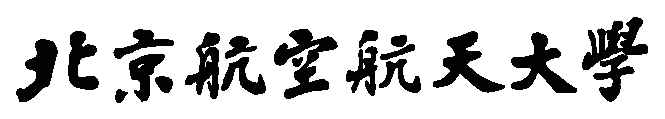
\includegraphics[width=.5\textwidth]{logo-buaa}
  \caption{测试图片\\第二行题注}
  \label{fig:logo}
\end{figure}
\centerline{-----------$\uparrow$-----------Space Check-----------$\uparrow$-----------}

我们在这儿插入一行字;

我们在这儿再插入一行字;

我们在这儿插入一行字;

我们在这儿再插入一行字;

我们在这儿插入一行字;

我们在这儿再插入一行字;

我们在这儿插入一行字;

我们在这儿再插入一行字;

\section{数学环境}

\subsection{数学符号}

模板定义了一些正体(upright)的数学符号:
\begin{center}
  \begin{tabular}{rl}
    \toprule
    符号                 & 命令 \\
    \midrule
    常数$\eu$     & \verb|\eu| \\
    复数单位$\iu$ & \verb|\iu| \\
    微分符号$\diff$ & \verb|\diff| \\
    $\argmax$         & \verb|\argmax| \\
    $\argmin$         & \verb|\argmin| \\
    \bottomrule
  \end{tabular}
\end{center}

更多的例子:
\begin{equation}
\eu^{\iu\pi} + 1 = 0
\end{equation}
\begin{equation}
\frac{\diff^2u}{\diff t^2} = \int f(x) \diff x
\end{equation}
\begin{equation}
\argmin_x f(x)
\end{equation}

\subsection{定理、引理和证明}

\begin{definition}
  If the integral of function $f$ is measurable and non-negative, we define
  its (extended) \textbf{Lebesgue integral} by
  \begin{equation}
  \int f = \sup_g \int g,
  \end{equation}
  where the supremum is taken over all measurable functions $g$ such that
  $0 \leq g \leq f$, and where $g$ is bounded and supported on a set of
  finite measure.
\end{definition}

\begin{example}
  Simple examples of functions on $\mathbf{R}^d$ that are integrable
  (or non-integrable) are given by
  \begin{equation}
  f_a(x) =
  \begin{cases}
  |x|^{-a} & \text{if } |x| \leq 1,\\
  0 & \text{if } x > 1.
  \end{cases}
  \end{equation}
  \begin{equation}
  F_a(x) = \frac{1}{1 + |x|^a}, \qquad \text{all } x \in \mathbf{R}^d.
  \end{equation}
  Then $f_a$ is integrable exactly when $a < d$, while $F_a$ is integrable
  exactly when $a > d$.
\end{example}

\begin{lemma}[Fatou]
  Suppose $\{f_n\}$ is a sequence of measurable functions with $f_n \geq 0$.
  If $\lim_{n \to \infty} f_n(x) = f(x)$ for a.e. $x$, then
  \begin{equation}
  \int f \leq \liminf_{n \to \infty} \int f_n.
  \end{equation}
\end{lemma}

\begin{remark}
  We do not exclude the cases $\int f = \infty$,
  or $\liminf_{n \to \infty} f_n = \infty$.
\end{remark}

\begin{corollary}
  Suppose $f$ is a non-negative measurable function, and $\{f_n\}$ a sequence
  of non-negative measurable functions with
  $f_n(x) \leq f(x)$ and $f_n(x) \to f(x)$ for almost every $x$. Then
  \begin{equation}
  \lim_{n \to \infty} \int f_n = \int f.
  \end{equation}
\end{corollary}

\begin{proposition}
  Suppose $f$ is integrable on $\mathbf{R}^d$. Then for every $\epsilon > 0$:
  \begin{enumerate}
    \renewcommand{\theenumi}{\roman{enumi}}
    \item There exists a set of finite measure $B$ (a ball, for example) such that
    \begin{equation}
    \int_{B^c} |f| < \epsilon.
    \end{equation}
    \item There is a $\delta > 0$ such that
    \begin{equation}
    \int_E |f| < \epsilon \qquad \text{whenever } m(E) < \delta.
    \end{equation}
  \end{enumerate}
\end{proposition}

\begin{theorem}
  Suppose $\{f_n\}$ is a sequence of measurable functions such that
  $f_n(x) \to f(x)$ a.e. $x$, as $n$ tends to infinity.
  If $|f_n(x)| \leq g(x)$, where $g$ is integrable, then
  \begin{equation}
  \int |f_n - f| \to 0 \qquad \text{as } n \to \infty,
  \end{equation}
  and consequently
  \begin{equation}
  \int f_n \to \int f \qquad \text{as } n \to \infty.
  \end{equation}
\end{theorem}

\begin{proof}
  Trivial.
\end{proof}



\subsection{自定义}

\newtheorem*{axiomofchoice}{Axiom of choice}
\begin{axiomofchoice}
  Suppose $E$ is a set and ${E_\alpha}$ is a collection of
  non-empty subsets of $E$. Then there is a function $\alpha
  \mapsto x_\alpha$ (a ``choice function'') such that
  \begin{equation}
  x_\alpha \in E_\alpha,\qquad \text{for all }\alpha.
  \end{equation}
\end{axiomofchoice}

\newtheorem{observation}{Observation}[chapter]
\begin{observation}
  Suppose a partially ordered set $P$ has the property
  that every chain has an upper bound in $P$. Then the
  set $P$ contains at least one maximal element.
\end{observation}
\begin{proof}[A concise proof]
  Obvious.
\end{proof}

\newtheorem{observationvar2}[observation]{Observationvar2}
\begin{observationvar2}
  Suppose a partially ordered set $P$ has the property
  that every chain has an upper bound in $P$. Then the
  set $P$ contains at least one maximal element.
\end{observationvar2}
\begin{proof}[A concise proof]
  Obvious.
\end{proof}

我们在这儿插入一行字;

我们在这儿再插入一行字;

我们在这儿插入一行字;

我们在这儿再插入一行字;

我们在这儿插入一行字;

我们在这儿再插入一行字;

我们在这儿插入一行字;

我们在这儿再插入一行字;

我们在这儿插入一行字;

我们在这儿再插入一行字;

我们在这儿插入一行字;

我们在这儿再插入一行字;

我们在这儿插入一行字;

我们在这儿再插入一行字;

我们在这儿插入一行字;

我们在这儿再插入一行字;

我们在这儿插入一行字;

我们在这儿再插入一行字;

% 总结
% !TeX root = ../Template.tex
% 总结
\summary
学位论文的结论单独作为一章,但不加章号。如果不可能导出应有的结论,也可以没有结论而进行必要的讨论。

\par * 嗯,这就是你的论文了 * \par


% 参考文献
% 2015版国标GBT7714-2015
% 2005版国标GBT7714-2005
\Bib{GBT7714-2015}{ref}

% 附录
% !TeX root = ../Template.tex
% [附录]
\appendix

下列内容可以作为附录:

\begin{enumerate}[label=\arabic*)]
\item 为了整篇论文材料的完整,但编入正文又有损于编排的条理和逻辑性,这一材料包括比正文更为详尽的信息、研究方法和技术更深入的叙述,建议可以阅读的参考文献题录,对了解正文内容有用的补充信息等;
\item 由于篇幅过大或取材于复制品而不便于编入正文的材料;
\item 不便于编入正文的罕见的珍贵或需要特别保密的技术细节和详细方案(这中情况可单列成册);
\item 对一般读者并非必要阅读,但对专业同行有参考价值的资料;
\item 某些重要的原始数据、过长的数学推导、计算程序、框图、结构图、注释、统计表、计算机打印输出文件等。
\end{enumerate}

\par * 嗯,自由发挥吧 * \par

% 攻读学位期间成果
% !TeX root = ../Template.tex
% [攻读学位期间取得的成果]
\achievement

对于博士学位论文,本条目名称用“攻读博士学位期间取得的研究成果”,一般包括:

攻读博士学位期间取得的学术成果:攻读博士学位期间取得的学术成果:列出攻读博士期间发表(含录用)的与学位论文相关的学位论文、发表专利、著作、获奖项目等,书写格式与参考文献格式相同;

攻读博士期间参与的主要科研项目:列出攻读博士学位期间参与的与学位论文相关的主要科研项目,包括项目名称,项目来源,研制时间,本人承担的主要工作。

对于硕士学位论文,本条目名称用“攻读硕士学位期间取得的学术成果”,只列出攻读硕士学位期间发表(含录用)的与学位论文相关的学位论文、发表专利、著作、获奖项目等,书写格式与参考文献格式相同。

\par * 嗯,研究生不列科研项目 * \par

% 致谢
% !TeX root = ../Template.tex
% [致谢]
\acknowledgments

致谢中主要感谢指导教师和在学术方面对论文的完成有直接贡献及重要帮助的团体和人士,以及感谢给予转载和引用权的资料、图片、文献、研究思想和设想的所有者。致谢中还可以感谢提供研究经费及实验装置的基金会或企业等单位和人士。致谢辞应谦虚诚恳,实事求是,切记浮夸与庸俗之词。

\par * 嗯,感谢完所有人之后,也请记得感谢一下自己 * \par

% 作者简介
% !TeX root = ../Template.tex
% [作者简介]
\biography
博士学位论文应该提供作者简介,主要包括:姓名、性别、出生年月日、民族、出生的;简要学历、工作经历(职务);以及攻读博士学位期间获得的其他奖项(除攻读学位期间取得的研究成果之外)。

\par * 嗯,“硕士学位论文无此项”,《手册》上是这么说的 * \par

\vspace{5cm}

This is \BUAAThesis{}, Happy TeXing! --- from WeiQM.

\end{document}
